% Options for packages loaded elsewhere
\PassOptionsToPackage{unicode}{hyperref}
\PassOptionsToPackage{hyphens}{url}
%
\documentclass[
]{book}
\usepackage{amsmath,amssymb}
\usepackage{lmodern}
\usepackage{iftex}
\ifPDFTeX
  \usepackage[T1]{fontenc}
  \usepackage[utf8]{inputenc}
  \usepackage{textcomp} % provide euro and other symbols
\else % if luatex or xetex
  \usepackage{unicode-math}
  \defaultfontfeatures{Scale=MatchLowercase}
  \defaultfontfeatures[\rmfamily]{Ligatures=TeX,Scale=1}
\fi
% Use upquote if available, for straight quotes in verbatim environments
\IfFileExists{upquote.sty}{\usepackage{upquote}}{}
\IfFileExists{microtype.sty}{% use microtype if available
  \usepackage[]{microtype}
  \UseMicrotypeSet[protrusion]{basicmath} % disable protrusion for tt fonts
}{}
\makeatletter
\@ifundefined{KOMAClassName}{% if non-KOMA class
  \IfFileExists{parskip.sty}{%
    \usepackage{parskip}
  }{% else
    \setlength{\parindent}{0pt}
    \setlength{\parskip}{6pt plus 2pt minus 1pt}}
}{% if KOMA class
  \KOMAoptions{parskip=half}}
\makeatother
\usepackage{xcolor}
\IfFileExists{xurl.sty}{\usepackage{xurl}}{} % add URL line breaks if available
\IfFileExists{bookmark.sty}{\usepackage{bookmark}}{\usepackage{hyperref}}
\hypersetup{
  pdftitle={Traitement des données PMSI avec R},
  pdfauthor={Guillaume Pressiat \textbar\textbar{} CHU Brest},
  hidelinks,
  pdfcreator={LaTeX via pandoc}}
\urlstyle{same} % disable monospaced font for URLs
\usepackage{color}
\usepackage{fancyvrb}
\newcommand{\VerbBar}{|}
\newcommand{\VERB}{\Verb[commandchars=\\\{\}]}
\DefineVerbatimEnvironment{Highlighting}{Verbatim}{commandchars=\\\{\}}
% Add ',fontsize=\small' for more characters per line
\usepackage{framed}
\definecolor{shadecolor}{RGB}{248,248,248}
\newenvironment{Shaded}{\begin{snugshade}}{\end{snugshade}}
\newcommand{\AlertTok}[1]{\textcolor[rgb]{0.94,0.16,0.16}{#1}}
\newcommand{\AnnotationTok}[1]{\textcolor[rgb]{0.56,0.35,0.01}{\textbf{\textit{#1}}}}
\newcommand{\AttributeTok}[1]{\textcolor[rgb]{0.77,0.63,0.00}{#1}}
\newcommand{\BaseNTok}[1]{\textcolor[rgb]{0.00,0.00,0.81}{#1}}
\newcommand{\BuiltInTok}[1]{#1}
\newcommand{\CharTok}[1]{\textcolor[rgb]{0.31,0.60,0.02}{#1}}
\newcommand{\CommentTok}[1]{\textcolor[rgb]{0.56,0.35,0.01}{\textit{#1}}}
\newcommand{\CommentVarTok}[1]{\textcolor[rgb]{0.56,0.35,0.01}{\textbf{\textit{#1}}}}
\newcommand{\ConstantTok}[1]{\textcolor[rgb]{0.00,0.00,0.00}{#1}}
\newcommand{\ControlFlowTok}[1]{\textcolor[rgb]{0.13,0.29,0.53}{\textbf{#1}}}
\newcommand{\DataTypeTok}[1]{\textcolor[rgb]{0.13,0.29,0.53}{#1}}
\newcommand{\DecValTok}[1]{\textcolor[rgb]{0.00,0.00,0.81}{#1}}
\newcommand{\DocumentationTok}[1]{\textcolor[rgb]{0.56,0.35,0.01}{\textbf{\textit{#1}}}}
\newcommand{\ErrorTok}[1]{\textcolor[rgb]{0.64,0.00,0.00}{\textbf{#1}}}
\newcommand{\ExtensionTok}[1]{#1}
\newcommand{\FloatTok}[1]{\textcolor[rgb]{0.00,0.00,0.81}{#1}}
\newcommand{\FunctionTok}[1]{\textcolor[rgb]{0.00,0.00,0.00}{#1}}
\newcommand{\ImportTok}[1]{#1}
\newcommand{\InformationTok}[1]{\textcolor[rgb]{0.56,0.35,0.01}{\textbf{\textit{#1}}}}
\newcommand{\KeywordTok}[1]{\textcolor[rgb]{0.13,0.29,0.53}{\textbf{#1}}}
\newcommand{\NormalTok}[1]{#1}
\newcommand{\OperatorTok}[1]{\textcolor[rgb]{0.81,0.36,0.00}{\textbf{#1}}}
\newcommand{\OtherTok}[1]{\textcolor[rgb]{0.56,0.35,0.01}{#1}}
\newcommand{\PreprocessorTok}[1]{\textcolor[rgb]{0.56,0.35,0.01}{\textit{#1}}}
\newcommand{\RegionMarkerTok}[1]{#1}
\newcommand{\SpecialCharTok}[1]{\textcolor[rgb]{0.00,0.00,0.00}{#1}}
\newcommand{\SpecialStringTok}[1]{\textcolor[rgb]{0.31,0.60,0.02}{#1}}
\newcommand{\StringTok}[1]{\textcolor[rgb]{0.31,0.60,0.02}{#1}}
\newcommand{\VariableTok}[1]{\textcolor[rgb]{0.00,0.00,0.00}{#1}}
\newcommand{\VerbatimStringTok}[1]{\textcolor[rgb]{0.31,0.60,0.02}{#1}}
\newcommand{\WarningTok}[1]{\textcolor[rgb]{0.56,0.35,0.01}{\textbf{\textit{#1}}}}
\usepackage{longtable,booktabs,array}
\usepackage{calc} % for calculating minipage widths
% Correct order of tables after \paragraph or \subparagraph
\usepackage{etoolbox}
\makeatletter
\patchcmd\longtable{\par}{\if@noskipsec\mbox{}\fi\par}{}{}
\makeatother
% Allow footnotes in longtable head/foot
\IfFileExists{footnotehyper.sty}{\usepackage{footnotehyper}}{\usepackage{footnote}}
\makesavenoteenv{longtable}
\usepackage{graphicx}
\makeatletter
\def\maxwidth{\ifdim\Gin@nat@width>\linewidth\linewidth\else\Gin@nat@width\fi}
\def\maxheight{\ifdim\Gin@nat@height>\textheight\textheight\else\Gin@nat@height\fi}
\makeatother
% Scale images if necessary, so that they will not overflow the page
% margins by default, and it is still possible to overwrite the defaults
% using explicit options in \includegraphics[width, height, ...]{}
\setkeys{Gin}{width=\maxwidth,height=\maxheight,keepaspectratio}
% Set default figure placement to htbp
\makeatletter
\def\fps@figure{htbp}
\makeatother
\setlength{\emergencystretch}{3em} % prevent overfull lines
\providecommand{\tightlist}{%
  \setlength{\itemsep}{0pt}\setlength{\parskip}{0pt}}
\setcounter{secnumdepth}{5}
%\usepackage{xcolor}
%\usepackage[usenames, , table]{xcolor}
% \usepackage{hyperref}
% \hypersetup{
%     colorlinks = true,
%     linkcolor = CadetBlue,
%     citecolor = CadetBlue,
%     urlcolor  = Blue,
%     linkbordercolor = gray,
%     allbordercolors = CornflowerBlue
% }
\usepackage{booktabs}
\usepackage{amsthm}
\renewcommand{\familydefault}{\sfdefault}
\renewcommand{\chaptername}{}
\renewcommand{\contentsname}{Tables des matières}



\makeatletter
\def\thm@space@setup{%
  \thm@preskip=8pt plus 2pt minus 4pt
  \thm@postskip=\thm@preskip
}
\makeatother
\ifLuaTeX
  \usepackage{selnolig}  % disable illegal ligatures
\fi
\usepackage[]{natbib}
\bibliographystyle{plainnat}

\title{Traitement des données PMSI avec R}
\author{Guillaume Pressiat \textbar\textbar{} CHU Brest}
\date{2021-11-21}

\begin{document}
\maketitle

{
\setcounter{tocdepth}{1}
\tableofcontents
}
\hypertarget{introduction}{%
\chapter{Introduction}\label{introduction}}

Ce livret numérique présente des exemples de traitements de données PMSI avec R. L'objectif est de concentrer ici :

\begin{itemize}
\item
  une documentation permettant de débuter avec l'import de données via le package \href{https://github.com/GuillaumePressiat/pmeasyr}{\emph{pmeasyr}}
\item
  des exemples d'analyses PMSI :

  \begin{itemize}
  \tightlist
  \item
    requêtes sur les diagnostics et les actes
  \item
    analyse des files actives pour une pathologie
  \item
    statistiques élementaires sur des variables du PMSI
  \item
    analyse du case-mix et de la dms par ghm
  \item
    valorisation des rsa
  \end{itemize}
\end{itemize}

\hypertarget{contexte}{%
\chapter{Contexte et motivations}\label{contexte}}

Les données du Programme de Médicalisation des Systèmes d'Information (PMSI) sont souvent traitées via des logiciels spécifiques au PMSI (ou des outils statistiques / bases de données du marché) ne permettant pas de réaliser des traitements statistiques et des infographies satisfaisantes. Les départements d'information médicale sont donc souvent amenés à retraiter ces données avec R.

L'évolution récente de R intègre la manipulation de bases de données de taille importante. Le package \emph{pmeasyr} s'inscrit dans cette veine et permet de réaliser de façon autonome l'ensemble des traitements (de l'import des données à leur analyse) avec R.

\hypertarget{avantages-de-r}{%
\section{Avantages de R}\label{avantages-de-r}}

\hypertarget{un-flux-de-travail-unique}{%
\subsection{Un flux de travail unique}\label{un-flux-de-travail-unique}}

En travaillant uniquement avec R, on peut mettre en place un flux de travail épuré : un seul projet, un seul programme, un seul logiciel. La traçabilité, la reproductibilité et la mise à jour des opérations sont ainsi facilitées.

Le travail avec de multiples logiciels oblige à l'export / import de fichiers entre les différents logiciels, et chaque modification du début du flux de travail génère des fichiers exportés v1, v2, \ldots{}

Avec un flux complet dans R, toute nouvelle modification est intégrée au processus de travail global. La localisation de toutes les étapes d'une analyse en un seul point évite les erreurs et la confusion lorsque l'on reprend l'analyse ultérieurement.

\hypertarget{r-et-le-pmsi}{%
\subsection{R et le PMSI}\label{r-et-le-pmsi}}

L'utilisation de R confère aux données du PMSI la liberté proposée par le logiciel :

\begin{itemize}
\tightlist
\item
  les requêtes sur les diagnostics et les actes peuvent s'écrire de multiples façons et c'est l'utilisateur qui crée ses propres programmes
\item
  les données sont dans R : prêtes pour des modèles linéaires, logistiques, des classifications\ldots{}
\item
  la confrontation des données in* (reflet du codage des établissements) aux données out* (reflet de la valorisation accordée à l'établissement) est facilitée par l'import du fichier tra, cela peut permettre aux équipes DIM d'améliorer leur recueil
\item
  le reporting de l'activité vers différents formats (Excel, PDF, Word, HTML) ou en créant des applications (\href{http://shiny.rstudio.com}{shiny})
\item
  l'utilisation des graphiques pour représenter des volumes d'activités et des cartographies interactives pour visualiser la localisation d'activités, de patientèles, et les flux de patients
\item
  le partage de projets RStudio, qui facilite et encourage les travaux en équipe.
\end{itemize}

\emph{NB: Données In / Out : données en entrée / sortie des logiciels de l'ATIH}

\hypertarget{des-outils-performants}{%
\subsection{Des outils performants}\label{des-outils-performants}}

L'engouement autour de R est lié au développement de packages intuitifs et performants : \href{http://readr.tidyverse.org}{\emph{readr}}, \href{https://github.com/hadley/dplyr}{\emph{dplyr}}, \href{http://tidyr.tidyverse.org}{\emph{tidyr}}, \href{https://github.com/tidyverse/magrittr}{\emph{magrittr}}, pour n'en citer que quelques-uns. \href{https://github.com/GuillaumePressiat/pmeasyr}{\emph{pmeasyr}} s'appuie sur ces packages pour proposer des imports de données rapides sur des fichiers de taille importante (l'entité juridique de l'AP-HP est prise en charge sans problème avec un ordinateur récent).

Dans le cas de \href{https://github.com/GuillaumePressiat/pmeasyr}{\emph{pmeasyr}}, l'import de 100 000 RSA (partie fixe, parsing des passages unités médicales, des diagnostics associés et des actes) nécessite en moyenne 5 secondes avec un processeur i7 -- 16Go de ram.

En dernier ressort, R travaillant en mémoire vive, les exécutions de requêtes sont très rapides.

\hypertarget{contenu-du-package}{%
\section{Contenu du package}\label{contenu-du-package}}

Le package contient des fonctions pour la gestion des archives PMSI en entrée / sortie des logiciels de l'ATIH : dézippage, suppression des archives, et des fonctions pour l'import des fichiers des champs PMSI MCO, SSR, HAD, PSY et RSF.

Il est utilisé depuis un an à l'AP-HP pour des analyses d'activité et la description des prises en charge.

\hypertarget{installation-du-package}{%
\section{Installation du package}\label{installation-du-package}}

\begin{Shaded}
\begin{Highlighting}[]
\NormalTok{remotes}\SpecialCharTok{::}\FunctionTok{install\_github}\NormalTok{(}\StringTok{\textquotesingle{}GuillaumePressiat/pmeasyr\textquotesingle{}}\NormalTok{)}
\end{Highlighting}
\end{Shaded}

Cette commande lance l'installation du package et de ses dépendances.

\hypertarget{archives}{%
\chapter{Les archives PMSI}\label{archives}}

Cette partie aborde le point de départ des études PMSI : les archives PMSI. Ces archives sont les fichiers en entrées / sorties des logiciels de l'ATIH.

Les manuels techniques de ces logiciels, relatifs aux champs MCO, SSR, HAD, PSY et RSF, respectivement \href{https://atih.sante.fr/plateformes-de-transmission-et-logiciels/logiciels-espace-de-telechargement\#G}{Genrsa}, \href{https://atih.sante.fr/plateformes-de-transmission-et-logiciels/logiciels-espace-de-telechargement\#G}{Genrha}, \href{https://atih.sante.fr/plateformes-de-transmission-et-logiciels/logiciels-espace-de-telechargement\#P}{Paprica}, \href{https://atih.sante.fr/plateformes-de-transmission-et-logiciels/logiciels-espace-de-telechargement\#P}{Pivoine} et \href{https://atih.sante.fr/plateformes-de-transmission-et-logiciels/logiciels-espace-de-telechargement\#P}{Preface} sont disponibles dans l'\href{https://atih.sante.fr/plateformes-de-transmission-et-logiciels/logiciels-espace-de-telechargement}{espace de téléchargement} sur le site de l'ATIH.

\hypertarget{arborescence-des-archives}{%
\section{Arborescence des archives}\label{arborescence-des-archives}}

Le package \emph{pmeasyr} prend en charge les données des quatre champs PMSI MCO, SSR, HAD, PSY ainsi que les RSF.

Placer les archives dans un répertoire, par exemple ici dans \texttt{\textasciitilde{}/Documents/data/mco} :

\begin{figure}
\centering
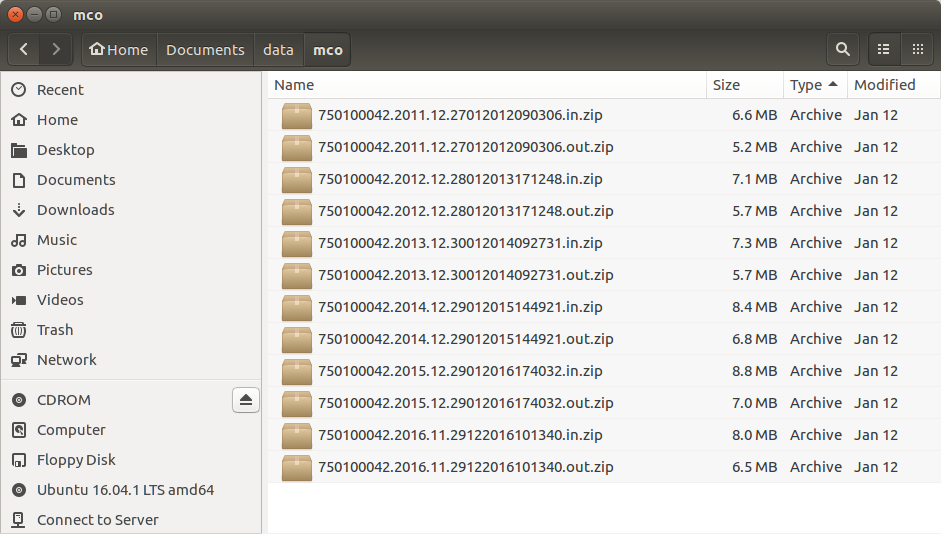
\includegraphics{images/archives_mco.png}
\caption{Archives MCO}
\end{figure}

Vous noterez que pour chaque champ PMSI il est conseillé d'utiliser un répertoire indépendant, ceci est nécessaire dans la mesure où le nom des archives PMSI ne contient pas l'information champ MCO, RSF, etc., il faut organiser l'archivage champ par champ, dans des répertoires différents.

\begin{figure}
\centering
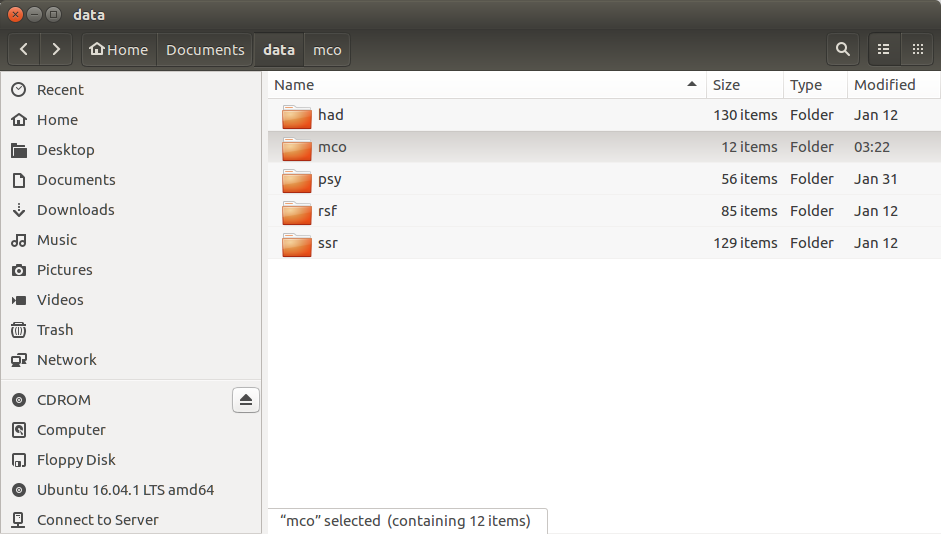
\includegraphics{images/champ_par_champ.png}
\caption{Un répertoire par champ PMSI}
\end{figure}

\begin{Shaded}
\begin{Highlighting}[]
\CommentTok{\# Créer l\textquotesingle{}arborescence à partir de R}
\NormalTok{champs }\OtherTok{=} \FunctionTok{c}\NormalTok{(}\StringTok{\textquotesingle{}mco\textquotesingle{}}\NormalTok{, }\StringTok{\textquotesingle{}ssr\textquotesingle{}}\NormalTok{, }\StringTok{\textquotesingle{}had\textquotesingle{}}\NormalTok{, }\StringTok{\textquotesingle{}psy\textquotesingle{}}\NormalTok{, }\StringTok{\textquotesingle{}rsf\textquotesingle{}}\NormalTok{)}
\NormalTok{emplacement }\OtherTok{\textless{}{-}} \StringTok{"\textasciitilde{}/Documents/data"}
\FunctionTok{sapply}\NormalTok{(champs, }\ControlFlowTok{function}\NormalTok{(x)\{}\FunctionTok{dir.create}\NormalTok{(}\FunctionTok{file.path}\NormalTok{(emplacement, x))\})}
\end{Highlighting}
\end{Shaded}

\hypertarget{sous-unix}{%
\subsection{Sous Unix}\label{sous-unix}}

Chaque utilisateur dispose de son path `\textasciitilde{}', qui équivaut par exemple à : `/home/gui/'.

\hypertarget{sous-windows}{%
\subsection{Sous Windows}\label{sous-windows}}

Chaque utilisateur dispose de son répertoire, exemple \texttt{C:/Users/gui/}. Et souvent, sans l'utilisation de projets RStudio, les chemins d'accès aux données sont pénibles à configurer dans chaque programme.

Mais dans R, le symbole `\textasciitilde{}' utilisé sur windows dans un chemin d'accès aux fichiers renvoie au répertoire Documents de l'utilisateur : \texttt{C:/Users/gui/Documents}.

\begin{Shaded}
\begin{Highlighting}[]
\FunctionTok{path.expand}\NormalTok{(}\StringTok{\textquotesingle{}\textasciitilde{}\textquotesingle{}}\NormalTok{)}
\end{Highlighting}
\end{Shaded}

renvoie \texttt{C:/Users/gui/Documents/}.

Par conséquent sur Windows le répertoire à créer pour localiser les fichiers d'archives pmsi sera : \texttt{C:/Users/gui/Documents/Documents/data}.

\textbf{N.B.: Nous proposons ici que les utilisateurs de \texttt{pmeasyr} utilisent ce chemin générique pour leurs programmes. L'avantage qui en découle : le partage de programme ne nécessite pas de changer le chemin d'accès, puisque c'est le même.}

\hypertarget{informations-sur-les-archives}{%
\section{Informations sur les archives}\label{informations-sur-les-archives}}

Le nom des fonctions dont l'objectif est de manipuler les \textbf{a}rchives commence par \textbf{a}.

La fonction \texttt{astat} permet d'éditer des statistiques sommaires sur les fichiers contenus dans une archive.

\begin{longtable}[]{@{}ll@{}}
\toprule
Nom & Fonction \\
\midrule
\endhead
\href{https://guillaumepressiat.github.io/pmeasyr/reference/astat.html}{astat} & \textasciitilde{} *.zip - Liste et volume des fichiers d'une archive PMSI \\
\bottomrule
\end{longtable}

\begin{Shaded}
\begin{Highlighting}[]
\CommentTok{\# Informations sur les fichiers : Date de creation, Taille}
\NormalTok{pmeasyr}\SpecialCharTok{::}\FunctionTok{astat}\NormalTok{(}\AttributeTok{path =} \StringTok{\textquotesingle{}\textasciitilde{}/Documents/data/mco/\textquotesingle{}}\NormalTok{, }
               \AttributeTok{file =} \StringTok{\textquotesingle{}750100042.2015.12.29012016174032.out.zip\textquotesingle{}}\NormalTok{, }
               \AttributeTok{view =}\NormalTok{ F)}
\end{Highlighting}
\end{Shaded}

\hypertarget{duxe9zippage}{%
\section{Dézippage}\label{duxe9zippage}}

Cette partie du package facilite la manipulation des archives PMSI, fichiers de type :

\begin{itemize}
\tightlist
\item
  \texttt{finess.annee.mois.date\_et\_heure\_de\_creation.in.zip}
\item
  \texttt{finess.annee.mois.date\_et\_heure\_de\_creation.out.zip}
\end{itemize}

Les fonctions permettent de dézipper les fichiers depuis \texttt{R} en ligne de commande, sans intervention manuelle de l'utilisateur. L'avantage est d'obtenir un processus ne relevant pas d'interventions externes au logiciel \texttt{R} (pour pouvoir garder trace des etapes, et faciliter la reproduction, tout est inscrit dans un programme, dans un flux de processus). Une fois que les traitements et analyses sur les fichiers sont faits, il est possible d'effacer les archives également en ligne de commande.

\begin{longtable}[]{@{}
  >{\raggedright\arraybackslash}p{(\columnwidth - 2\tabcolsep) * \real{0.1031}}
  >{\raggedright\arraybackslash}p{(\columnwidth - 2\tabcolsep) * \real{0.8969}}@{}}
\toprule
\begin{minipage}[b]{\linewidth}\raggedright
Nom
\end{minipage} & \begin{minipage}[b]{\linewidth}\raggedright
Fonction
\end{minipage} \\
\midrule
\endhead
\href{https://guillaumepressiat.github.io/pmeasyr/reference/adezip.html}{adezip} & \textasciitilde{} *.zip - Dezippe des fichiers de l'archive PMSI \\
\href{https://guillaumepressiat.github.io/pmeasyr/reference/adezip2.html}{adezip2} & \textasciitilde{} *.zip - Dezippe des fichiers de l'archive PMSI, avec en parametre le nom de l'archive \\
\bottomrule
\end{longtable}

\begin{Shaded}
\begin{Highlighting}[]
\CommentTok{\# Dezippage uniquement des fichiers rsa, ano et tra du out 2015}
\CommentTok{\# Ex: 750100042.2015.12.20160130.153012.out.zip}
\NormalTok{pmeasyr}\SpecialCharTok{::}\FunctionTok{adezip}\NormalTok{(}\AttributeTok{finess =} \DecValTok{750100042}\NormalTok{, }
                \AttributeTok{annee =} \DecValTok{2015}\NormalTok{, }
                \AttributeTok{mois =} \DecValTok{12}\NormalTok{, }
                \AttributeTok{path =} \StringTok{\textquotesingle{}\textasciitilde{}/Documents/data/mco\textquotesingle{}}\NormalTok{, }
                \AttributeTok{liste =} \FunctionTok{c}\NormalTok{(}\StringTok{"rsa"}\NormalTok{, }\StringTok{"ano"}\NormalTok{, }\StringTok{"tra"}\NormalTok{), }
                \AttributeTok{type =} \StringTok{"out"}\NormalTok{)}
\end{Highlighting}
\end{Shaded}

\begin{figure}
\centering
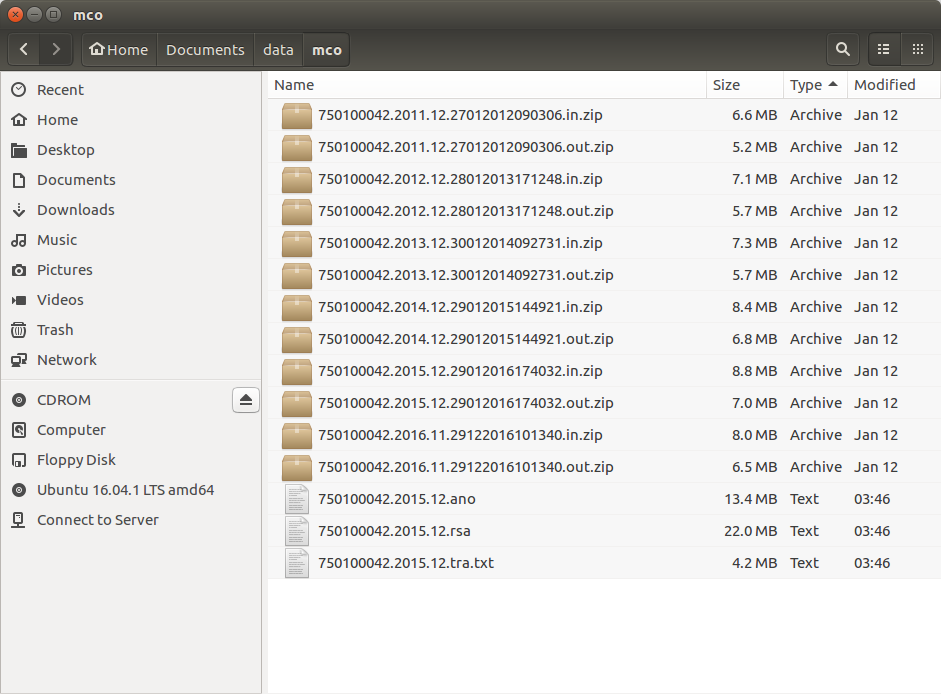
\includegraphics{images/archives_dezip.png}
\caption{Après éxécution de \texttt{adezip()} sur des fichiers du \emph{out}}
\end{figure}

\begin{Shaded}
\begin{Highlighting}[]
\CommentTok{\# Dezippage uniquement des fichiers rss, dmi et med du in 2015}
\CommentTok{\# Ex: 750100042.2015.12.20160130.153012.out.zip}
\NormalTok{pmeasyr}\SpecialCharTok{::}\FunctionTok{adezip}\NormalTok{(}\AttributeTok{finess =} \DecValTok{750100042}\NormalTok{, }
                \AttributeTok{annee =} \DecValTok{2015}\NormalTok{, }
                \AttributeTok{mois =} \DecValTok{12}\NormalTok{, }
                \AttributeTok{path =} \StringTok{\textquotesingle{}\textasciitilde{}/Documents/data/mco\textquotesingle{}}\NormalTok{, }
                \AttributeTok{liste =} \FunctionTok{c}\NormalTok{(}\StringTok{"rss"}\NormalTok{, }\StringTok{"dmi"}\NormalTok{, }\StringTok{"med"}\NormalTok{), }
                \AttributeTok{type =} \StringTok{"in"}\NormalTok{)}
\end{Highlighting}
\end{Shaded}

\begin{figure}
\centering
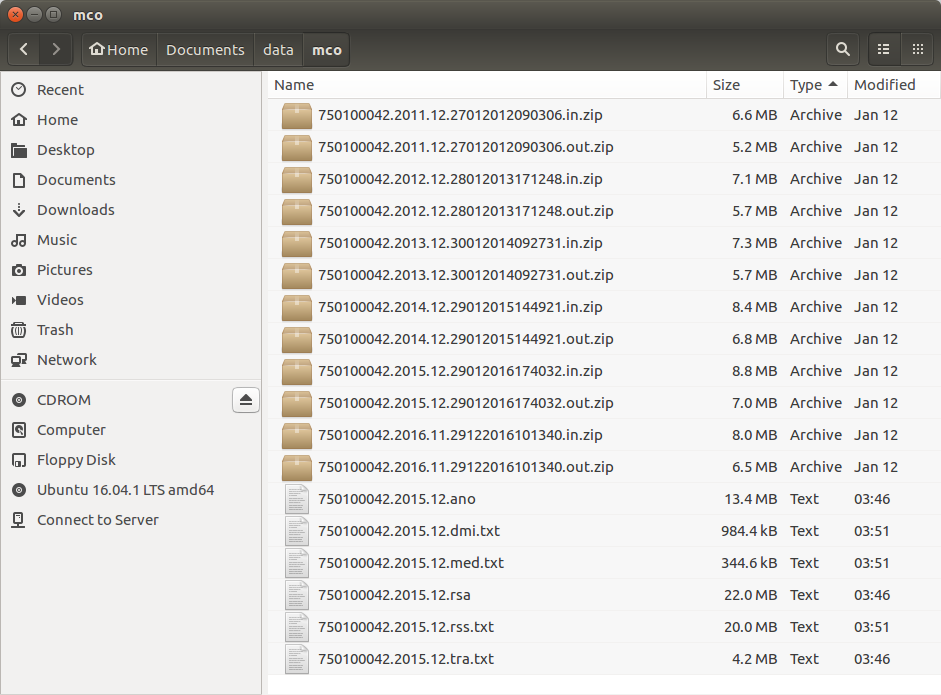
\includegraphics{images/archives_mco_in.png}
\caption{Après éxécution de \texttt{adezip()} sur des fichiers du \emph{in}}
\end{figure}

\hypertarget{suppression}{%
\section{Suppression}\label{suppression}}

À la fin d'une étude, il est inutile de garder les fichiers dézippés hors de l'archive, on peut les effacer : c'est ce que permet la fonction \texttt{adelete()}.

\begin{Shaded}
\begin{Highlighting}[]
\CommentTok{\# Effacer les fichiers}
\NormalTok{pmeasyr}\SpecialCharTok{::}\FunctionTok{adelete}\NormalTok{(}\AttributeTok{finess =} \DecValTok{750100042}\NormalTok{, }
                 \AttributeTok{annee =} \DecValTok{2015}\NormalTok{, }
                 \AttributeTok{mois =} \DecValTok{12}\NormalTok{, }
                 \AttributeTok{path =} \StringTok{\textquotesingle{}\textasciitilde{}/Documents/data/mco\textquotesingle{}}\NormalTok{, }
                 \AttributeTok{liste =} \FunctionTok{c}\NormalTok{(}\StringTok{"rsa"}\NormalTok{, }\StringTok{"ano"}\NormalTok{, }\StringTok{"tra"}\NormalTok{), }
                 \AttributeTok{type =} \StringTok{"out"}\NormalTok{)}

\NormalTok{pmeasyr}\SpecialCharTok{::}\FunctionTok{adelete}\NormalTok{(}\AttributeTok{finess =} \DecValTok{750100042}\NormalTok{, }
                 \AttributeTok{annee =} \DecValTok{2015}\NormalTok{, }
                 \AttributeTok{mois =} \DecValTok{12}\NormalTok{, }
                 \AttributeTok{path =} \StringTok{\textquotesingle{}\textasciitilde{}/Documents/data/mco\textquotesingle{}}\NormalTok{, }
                 \AttributeTok{liste =} \FunctionTok{c}\NormalTok{(}\StringTok{"rss"}\NormalTok{, }\StringTok{"med"}\NormalTok{, }\StringTok{"dmi"}\NormalTok{), }
                 \AttributeTok{type =} \StringTok{"in"}\NormalTok{)}
\end{Highlighting}
\end{Shaded}

\begin{figure}
\centering
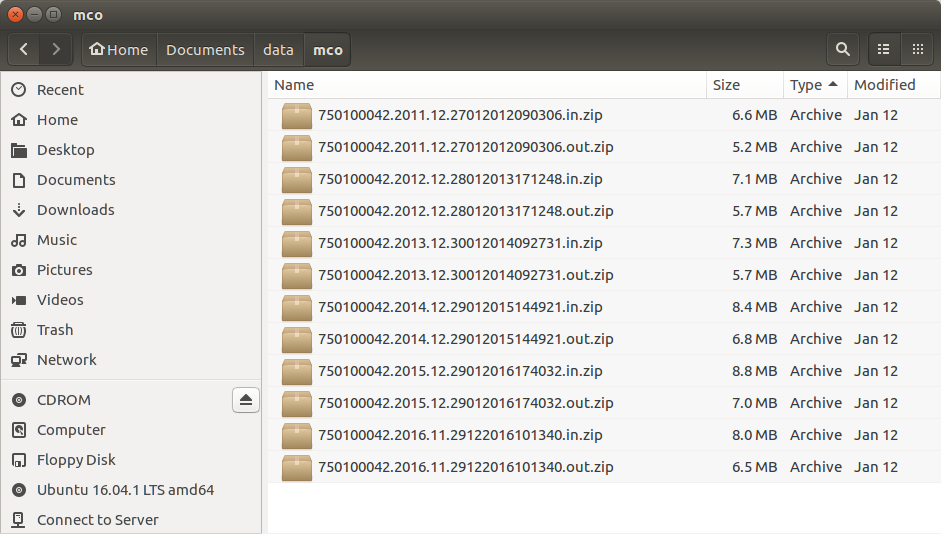
\includegraphics{images/archives_mco.png}
\caption{Après éxécution de \texttt{adelete()}}
\end{figure}

\hypertarget{import-des-donnuxe9es}{%
\chapter{Import des données}\label{import-des-donnuxe9es}}

\hypertarget{mco}{%
\section{MCO}\label{mco}}

\begin{longtable}[]{@{}ll@{}}
\toprule
Nom & Fonction \\
\midrule
\endhead
\href{https://guillaumepressiat.github.io/pmeasyr/reference/irsa.html}{irsa} & \textasciitilde{} MCO - Import des RSA \\
\href{https://guillaumepressiat.github.io/pmeasyr/reference/irum.html}{irum} & \textasciitilde{} MCO - Import des RUM \\
\href{https://guillaumepressiat.github.io/pmeasyr/reference/idiap.html}{idiap} & \textasciitilde{} MCO - Import des DIAP \\
\href{https://guillaumepressiat.github.io/pmeasyr/reference/idmi_mco.html}{idmi\_mco} & \textasciitilde{} MCO - Import des DMI \\
\href{https://guillaumepressiat.github.io/pmeasyr/reference/iium.html}{iium} & \textasciitilde{} MCO - Import des donnees UM \\
\href{https://guillaumepressiat.github.io/pmeasyr/reference/ileg_mco.html}{ileg\_mco} & \textasciitilde{} MCO - Import des erreurs Leg \\
\href{https://guillaumepressiat.github.io/pmeasyr/reference/imed_mco.html}{imed\_mco} & \textasciitilde{} MCO - Import des Med \\
\href{https://guillaumepressiat.github.io/pmeasyr/reference/ipo.html}{ipo} & \textasciitilde{} MCO - Import des PO \\
\href{https://guillaumepressiat.github.io/pmeasyr/reference/iano_mco.html}{iano\_mco} & \textasciitilde{} MCO - Import des Anohosp \\
\bottomrule
\end{longtable}

Les données in / out sont prises en charge.

\hypertarget{rsa}{%
\subsection{RSA}\label{rsa}}

Selon la nature des analyses à produire, plusieurs types d'imports sont possibles :

\begin{longtable}[]{@{}
  >{\raggedleft\arraybackslash}p{(\columnwidth - 2\tabcolsep) * \real{0.0556}}
  >{\raggedright\arraybackslash}p{(\columnwidth - 2\tabcolsep) * \real{0.9444}}@{}}
\toprule
\begin{minipage}[b]{\linewidth}\raggedleft
Type
\end{minipage} & \begin{minipage}[b]{\linewidth}\raggedright
Import
\end{minipage} \\
\midrule
\endhead
1 & Light : Partie fixe \\
2 & Light+ : Partie fixe + stream en ligne (+) actes et das \\
3 & Light++ : Partie fixe + stream en ligne (++) actes, das, typaut um et dpdr des um \\
4 & Standard : Partie fixe + creation des tables actes, das et rsa\_um \\
5 & Standard+ : Partie fixe + creation des tables actes, das et rsa\_um + stream (+) \\
6 & Standard++ : Partie fixe + creation des tables actes, das et rsa\_um + stream (++) \\
\bottomrule
\end{longtable}

\begin{Shaded}
\begin{Highlighting}[]
\FunctionTok{library}\NormalTok{(pmeasyr)}
\CommentTok{\# Import des rsa 2015 type 6}
\FunctionTok{irsa}\NormalTok{(}\AttributeTok{finess =} \DecValTok{750100042}\NormalTok{, }
     \AttributeTok{annee =} \DecValTok{2015}\NormalTok{, }
     \AttributeTok{mois =} \DecValTok{12}\NormalTok{, }
     \AttributeTok{path =} \StringTok{\textquotesingle{}\textasciitilde{}/Documents/data/mco\textquotesingle{}}\NormalTok{, }
     \AttributeTok{typi =} \DecValTok{6}\NormalTok{) }\OtherTok{{-}\textgreater{}}\NormalTok{ rsa15}
\FunctionTok{View}\NormalTok{(rsa15}\SpecialCharTok{$}\NormalTok{rsa)}
\FunctionTok{View}\NormalTok{(rsa15}\SpecialCharTok{$}\NormalTok{rsa\_um)}
\FunctionTok{View}\NormalTok{(rsa15}\SpecialCharTok{$}\NormalTok{actes)}
\FunctionTok{View}\NormalTok{(rsa15}\SpecialCharTok{$}\NormalTok{das)}
\end{Highlighting}
\end{Shaded}

Les tables sont par défaut avec des libellés :

\begin{figure}
\centering
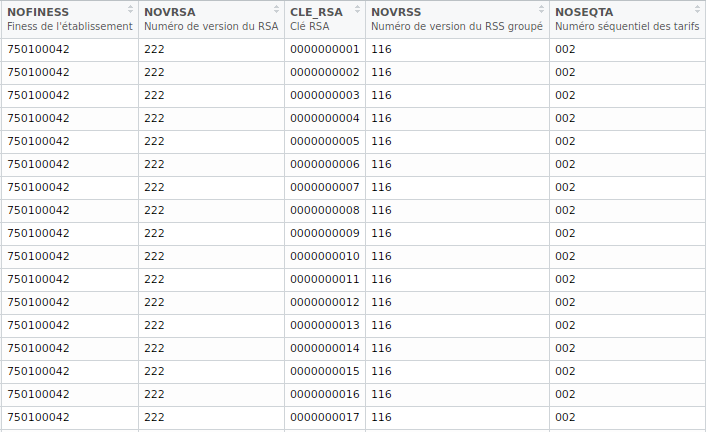
\includegraphics{images/rsa1.png}
\caption{Capture d'une portion de la table \texttt{rsa15\$rsa}}
\end{figure}

\hypertarget{rum}{%
\subsection{RUM}\label{rum}}

\begin{Shaded}
\begin{Highlighting}[]
\CommentTok{\# Import des rum 2015}
\FunctionTok{irum}\NormalTok{(}\AttributeTok{finess =} \DecValTok{750100042}\NormalTok{, }
     \AttributeTok{annee =} \DecValTok{2015}\NormalTok{, }
     \AttributeTok{mois =} \DecValTok{12}\NormalTok{, }
     \AttributeTok{path =} \StringTok{\textquotesingle{}\textasciitilde{}/Documents/data/mco\textquotesingle{}}\NormalTok{)}
\end{Highlighting}
\end{Shaded}

Selon la nature des analyses à produire, plusieurs types d'imports sont possibles :

\begin{longtable}[]{@{}rl@{}}
\toprule
Type & Import \\
\midrule
\endhead
1 & XLight : Partie fixe \\
2 & Light : Partie fixe + stream en ligne des actes, das et dad \\
3 & Standard : Partie fixe + table actes, das, dad \\
4 & Standard+ : Partie fixe + stream + table actes, das, dad \\
\bottomrule
\end{longtable}

\hypertarget{colonnes-stream}{%
\subsection{Colonnes stream}\label{colonnes-stream}}

\textbf{Exemples sur quelques rsa} :

\begin{itemize}
\tightlist
\item
  actes : Actes CCAM du Rsa
\end{itemize}

\begin{longtable}[]{@{}rl@{}}
\toprule
Cle RSA & actes \\
\midrule
\endhead
0000000001 & EDSF004, EDSF004, JQGA004, JQGA004 \\
0000000002 & EPLF002, DEQP003, DEQP007, DZQM006 \\
0000000003 & EBQH002, EEQH002, YYYY180 \\
\bottomrule
\end{longtable}

\begin{itemize}
\tightlist
\item
  dpdrum : zones diagnostics des passages UM du Rsa
\end{itemize}

\begin{longtable}[]{@{}rl@{}}
\toprule
Cle RSA & dpdrum \\
\midrule
\endhead
0000000004 & Z098 I671 \\
0000000005 & Z380, P741, Z380 \\
\bottomrule
\end{longtable}

\begin{itemize}
\tightlist
\item
  das : zones diagnostics associes du Rsa
\end{itemize}

\begin{longtable}[]{@{}rl@{}}
\toprule
Cle RSA & das \\
\midrule
\endhead
0000000006 & Z9580, Z9588 \\
0000000007 & P011, P032, P036, P011, P032, P700, P011, P032, P036 \\
\bottomrule
\end{longtable}

\begin{itemize}
\tightlist
\item
  um : types autorisations T2A des um de passage par ordre chronologique
\end{itemize}

\begin{longtable}[]{@{}rl@{}}
\toprule
Cle RSA & um \\
\midrule
\endhead
0000000009 & 01AC, 53 C \\
0000000010 & 51 C \\
0000000011 & 71 C, 04 C, 71 C \\
\bottomrule
\end{longtable}

\begin{figure}
\centering
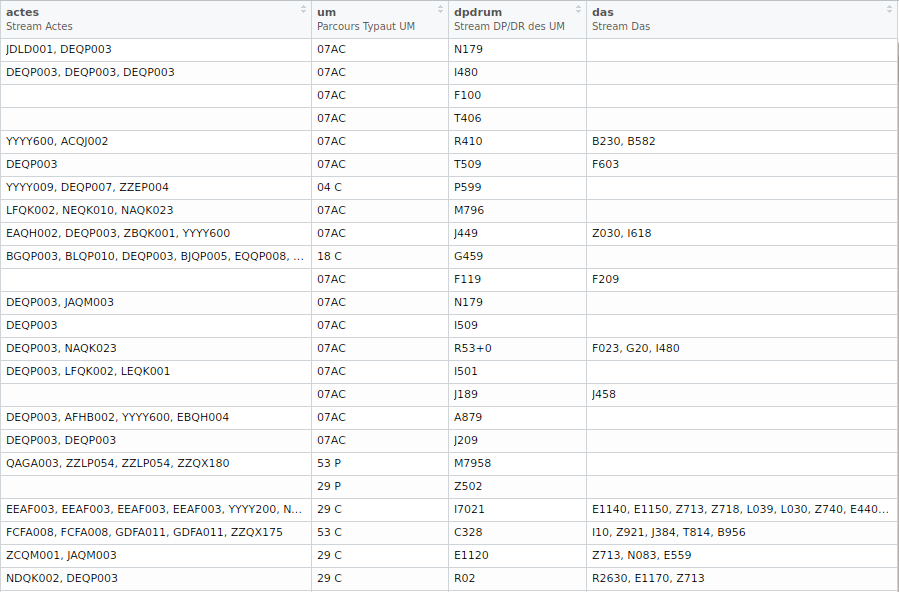
\includegraphics{images/rsa_stream.png}
\caption{Capture des zones \emph{stream} de la table \texttt{rsa15\$rsa}}
\end{figure}

Pour les quatre autres champs PMSI, seules les données du \emph{out} sont prises en charge par le package pour le moment.

Les fonctions d'imports pour ces champs PMSI reposent sur le même principe qu'en MCO.

\hypertarget{had}{%
\section{HAD}\label{had}}

\begin{longtable}[]{@{}ll@{}}
\toprule
Nom & Fonction \\
\midrule
\endhead
\href{https://guillaumepressiat.github.io/pmeasyr/reference/iano_had.html}{iano\_had} & \textasciitilde{} HAD - Import des Anohosp \\
\href{https://guillaumepressiat.github.io/pmeasyr/reference/imed_had.html}{imed\_had} & \textasciitilde{} HAD - Import des Med \\
\href{https://guillaumepressiat.github.io/pmeasyr/reference/irapss.html}{irapss} & \textasciitilde{} HAD - Import des RAPSS \\
\href{https://guillaumepressiat.github.io/pmeasyr/reference/ileg_had.html}{ileg\_had} & \textasciitilde{} HAD - Import des erreurs LEG \\
\bottomrule
\end{longtable}

\begin{Shaded}
\begin{Highlighting}[]
\FunctionTok{library}\NormalTok{(pmeasyr)}
\CommentTok{\# Import des rapss 2015}
\FunctionTok{irapss}\NormalTok{(}\AttributeTok{finess =} \DecValTok{750712184}\NormalTok{,}
       \AttributeTok{annee =} \DecValTok{2015}\NormalTok{,}
       \AttributeTok{mois =} \DecValTok{12}\NormalTok{,}
       \AttributeTok{path =} \StringTok{\textquotesingle{}\textasciitilde{}/Documents/data/had\textquotesingle{}}\NormalTok{) }\OtherTok{{-}\textgreater{}}\NormalTok{ data\_had}
\end{Highlighting}
\end{Shaded}

\hypertarget{ssr}{%
\section{SSR}\label{ssr}}

\begin{longtable}[]{@{}ll@{}}
\toprule
Nom & Fonction \\
\midrule
\endhead
\href{https://guillaumepressiat.github.io/pmeasyr/reference/iano_ssr.html}{iano\_ssr} & \textasciitilde{} SSR - Import des Anohosp \\
\href{https://guillaumepressiat.github.io/pmeasyr/reference/irha.html}{irha} & \textasciitilde{} SSR - Import des RHA \\
\href{https://guillaumepressiat.github.io/pmeasyr/reference/issrha.html}{issrha} & \textasciitilde{} SSR - Import des SSRHA \\
\href{https://guillaumepressiat.github.io/pmeasyr/reference/imed_ssr.html}{imed\_ssr} & \textasciitilde{} SSR - Import des MED \\
\href{https://guillaumepressiat.github.io/pmeasyr/reference/iium_ssr.html}{iium\_ssr} & \textasciitilde{} SSR - Import des UM \\
\href{https://guillaumepressiat.github.io/pmeasyr/reference/ileg_ssr.html}{ileg\_ssr} & \textasciitilde{} SSR - Import des erreurs LEG \\
\bottomrule
\end{longtable}

\begin{Shaded}
\begin{Highlighting}[]
\CommentTok{\# Import des rha 2015}
\FunctionTok{irha}\NormalTok{(}\AttributeTok{finess =} \DecValTok{750041543}\NormalTok{,}
     \AttributeTok{annee =} \DecValTok{2015}\NormalTok{,}
     \AttributeTok{mois =} \DecValTok{12}\NormalTok{,}
     \AttributeTok{path =} \StringTok{\textquotesingle{}\textasciitilde{}/Documents/data/ssr\textquotesingle{}}\NormalTok{) }\OtherTok{{-}\textgreater{}}\NormalTok{ data\_ssr}
\end{Highlighting}
\end{Shaded}

\hypertarget{psy}{%
\section{PSY}\label{psy}}

\begin{longtable}[]{@{}ll@{}}
\toprule
Nom & Fonction \\
\midrule
\endhead
\href{https://guillaumepressiat.github.io/pmeasyr/reference/iano_psy.html}{iano\_psy} & \textasciitilde{} PSY - Import des Anohosp \\
\href{https://guillaumepressiat.github.io/pmeasyr/reference/ir3a.html}{ir3a} & \textasciitilde{} PSY - Import des R3A \\
\href{https://guillaumepressiat.github.io/pmeasyr/reference/irpsa.html}{irpsa} & \textasciitilde{} PSY - Import des RPSA \\
\bottomrule
\end{longtable}

\begin{Shaded}
\begin{Highlighting}[]
\CommentTok{\# Import des rpsa 2015}
\FunctionTok{irpsa}\NormalTok{(}\AttributeTok{finess =} \DecValTok{750803454}\NormalTok{,}
      \AttributeTok{annee =} \DecValTok{2015}\NormalTok{,}
      \AttributeTok{mois =} \DecValTok{12}\NormalTok{,}
      \AttributeTok{path =} \StringTok{\textquotesingle{}\textasciitilde{}/Documents/data/psy\textquotesingle{}}\NormalTok{) }\OtherTok{{-}\textgreater{}}\NormalTok{ rpsa\_psy}

\CommentTok{\# Import des r3a 2015}
\FunctionTok{ir3a}\NormalTok{(}\AttributeTok{finess =} \DecValTok{750803454}\NormalTok{,}
      \AttributeTok{annee =} \DecValTok{2015}\NormalTok{,}
      \AttributeTok{mois =} \DecValTok{12}\NormalTok{,}
      \AttributeTok{path =} \StringTok{\textquotesingle{}\textasciitilde{}/Documents/data/psy\textquotesingle{}}\NormalTok{) }\OtherTok{{-}\textgreater{}}\NormalTok{ r3a\_psy}
\end{Highlighting}
\end{Shaded}

\hypertarget{rsf}{%
\section{RSF}\label{rsf}}

\begin{longtable}[]{@{}ll@{}}
\toprule
Nom & Fonction \\
\midrule
\endhead
\href{https://guillaumepressiat.github.io/pmeasyr/reference/irafael.html}{irafael} & \textasciitilde{} RSF - Import des RSFA / Rafael \\
\href{https://guillaumepressiat.github.io/pmeasyr/reference/iano_rafael.html}{iano\_rafael} & \textasciitilde{} RSF - Import des RSFA / ANO \\
\bottomrule
\end{longtable}

\begin{Shaded}
\begin{Highlighting}[]
\CommentTok{\# Import des rsfa 2015}
\FunctionTok{irafael}\NormalTok{(}\AttributeTok{finess =} \DecValTok{750712184}\NormalTok{,}
        \AttributeTok{annee =} \DecValTok{2015}\NormalTok{,}
        \AttributeTok{mois =} \DecValTok{12}\NormalTok{,}
        \AttributeTok{path =} \StringTok{\textquotesingle{}\textasciitilde{}/Documents/data/rsf\textquotesingle{}}\NormalTok{) }\OtherTok{{-}\textgreater{}}\NormalTok{ rsfa}
\end{Highlighting}
\end{Shaded}

\hypertarget{dictionnaire-de-variables}{%
\section{Dictionnaire de variables}\label{dictionnaire-de-variables}}

\begin{Shaded}
\begin{Highlighting}[]
\CommentTok{\# Obtenir les noms, labels et types de variables (character, numeric, integer, date, ...)}
\FunctionTok{dico}\NormalTok{(rsa15}\SpecialCharTok{$}\NormalTok{rsa)}
\end{Highlighting}
\end{Shaded}

\begin{Shaded}
\begin{Highlighting}[]
\CommentTok{\# Charger les formats de toutes les tables prises en charge par le package}
\NormalTok{pmeasyr}\SpecialCharTok{::}\NormalTok{formats}
\end{Highlighting}
\end{Shaded}

\hypertarget{labels}{%
\section{Labels}\label{labels}}

\begin{Shaded}
\begin{Highlighting}[]
\CommentTok{\# Obtenir le libelle d\textquotesingle{}une variable du PMSI}
\FunctionTok{labeleasier}\NormalTok{(rsa15}\SpecialCharTok{$}\NormalTok{rsa}\SpecialCharTok{$}\NormalTok{SEXE, }\AttributeTok{Sexe =}\NormalTok{ T)}
\FunctionTok{labeleasier}\NormalTok{(rsa15}\SpecialCharTok{$}\NormalTok{rsa}\SpecialCharTok{$}\NormalTok{ECHPMSI, }\AttributeTok{Mode\_entree =}\NormalTok{ T)}
\end{Highlighting}
\end{Shaded}

\hypertarget{requuxeates-sur-des-pathologies-actes}{%
\chapter{Requêtes sur des pathologies / actes}\label{requuxeates-sur-des-pathologies-actes}}

\hypertarget{transposition-des-codes-diagnostics}{%
\section{Transposition des codes diagnostics}\label{transposition-des-codes-diagnostics}}

Les analyses sur les diagnostics CIM-10 sont parfois fastidieuses du fait des multiples positions de diagnostics : DP principal du séjour, DR principal du séjour, DPUM, DRUM, DAS. La fonction \emph{tdiag} permet de rassembler tous les diagnostics dans une seule table.

\begin{Shaded}
\begin{Highlighting}[]
\CommentTok{\# Pour les objets rsa et rum du MCO}
\CommentTok{\# Transbahuter tous les diagnostics dans une seule table}
\FunctionTok{tdiag}\NormalTok{(rsa15) }\OtherTok{{-}\textgreater{}}\NormalTok{ rsa15 }\CommentTok{\# "Tidy diagnostics"}
\FunctionTok{View}\NormalTok{(rsa15}\SpecialCharTok{$}\NormalTok{diags)}
\CommentTok{\# Tous les diagnostics sont dans une table, avec un numero selon leur position  }
\CommentTok{\# 1:DP, 2:DR, 3:DPUM, 4:DRUM, 5:DAS}
\end{Highlighting}
\end{Shaded}

Exemple de résultat :

\begin{longtable}[]{@{}llll@{}}
\toprule
CLE\_RSA & NSEQRUM & position & diag \\
\midrule
\endhead
0000000001 & 01 & 1 & Z511 \\
0000000001 & 01 & 2 & C18 \\
0000000002 & 01 & 1 & C501 \\
0000000002 & 01 & 3 & C501 \\
0000000002 & 02 & 1 & D051 \\
0000000002 & 02 & 5 & E109 \\
\bottomrule
\end{longtable}

\hypertarget{recherche-de-codes-diagnostics}{%
\section{Recherche de codes diagnostics}\label{recherche-de-codes-diagnostics}}

L'objectif est de récupérer les séjours présentant un code diagnostic de la liste

\begin{Shaded}
\begin{Highlighting}[]
\CommentTok{\# Liste D{-}0103 de la fonction groupage 2016 : Epilepsies}
\NormalTok{liste\_diag }\OtherTok{=} \FunctionTok{c}\NormalTok{(}\StringTok{\textquotesingle{}F803\textquotesingle{}}\NormalTok{, }\StringTok{\textquotesingle{}G400\textquotesingle{}}\NormalTok{, }\StringTok{\textquotesingle{}G401\textquotesingle{}}\NormalTok{, }\StringTok{\textquotesingle{}G402\textquotesingle{}}\NormalTok{, }\StringTok{\textquotesingle{}G403\textquotesingle{}}\NormalTok{, }\StringTok{\textquotesingle{}G404\textquotesingle{}}\NormalTok{, }
               \StringTok{\textquotesingle{}G405\textquotesingle{}}\NormalTok{, }\StringTok{\textquotesingle{}G406\textquotesingle{}}\NormalTok{, }\StringTok{\textquotesingle{}G407\textquotesingle{}}\NormalTok{, }\StringTok{\textquotesingle{}G408\textquotesingle{}}\NormalTok{, }\StringTok{\textquotesingle{}G409\textquotesingle{}}\NormalTok{, }\StringTok{\textquotesingle{}G410\textquotesingle{}}\NormalTok{, }
               \StringTok{\textquotesingle{}G411\textquotesingle{}}\NormalTok{, }\StringTok{\textquotesingle{}G412\textquotesingle{}}\NormalTok{, }\StringTok{\textquotesingle{}G418\textquotesingle{}}\NormalTok{, }\StringTok{\textquotesingle{}G419\textquotesingle{}}\NormalTok{, }\StringTok{\textquotesingle{}R568\textquotesingle{}}\NormalTok{)}

\CommentTok{\# En passant par la table diags}
\FunctionTok{tdiag}\NormalTok{(rsa15) }\OtherTok{{-}\textgreater{}}\NormalTok{ rsa15}

\FunctionTok{library}\NormalTok{(dplyr)}
\CommentTok{\# quelle que soit la position du diagnostic}
\NormalTok{rsa15}\SpecialCharTok{$}\NormalTok{diags }\SpecialCharTok{\%\textgreater{}\%} \FunctionTok{filter}\NormalTok{(diag }\SpecialCharTok{\%in\%}\NormalTok{ liste\_diag)}
\CommentTok{\# position en das}
\NormalTok{rsa15}\SpecialCharTok{$}\NormalTok{diags }\SpecialCharTok{\%\textgreater{}\%} \FunctionTok{filter}\NormalTok{(diag }\SpecialCharTok{\%in\%}\NormalTok{ liste\_diag, position }\SpecialCharTok{==} \DecValTok{5}\NormalTok{)}
\CommentTok{\# position en dp dr}
\NormalTok{rsa15}\SpecialCharTok{$}\NormalTok{diags }\SpecialCharTok{\%\textgreater{}\%} \FunctionTok{filter}\NormalTok{(diag }\SpecialCharTok{\%in\%}\NormalTok{ liste\_diag, position }\SpecialCharTok{\textless{}} \DecValTok{5}\NormalTok{)}

\CommentTok{\# En passant par les zones stream}
\NormalTok{string\_diags }\OtherTok{=} 
  \StringTok{\textquotesingle{}F803|G400|G401|G402|G403|G404|G405|G406|G407|G408|G409|G410|G411|G412|G418|G419|R568\textquotesingle{}}

\CommentTok{\# quelle que soit la position du diagnostic}
\NormalTok{rsa15}\SpecialCharTok{$}\NormalTok{rsa }\SpecialCharTok{\%\textgreater{}\%} \FunctionTok{filter}\NormalTok{(}\FunctionTok{grepl}\NormalTok{(string\_diags, dpdrum)}\SpecialCharTok{|}\FunctionTok{grepl}\NormalTok{(string\_diags, das))}
\CommentTok{\# position en das}
\NormalTok{rsa15}\SpecialCharTok{$}\NormalTok{rsa }\SpecialCharTok{\%\textgreater{}\%} \FunctionTok{filter}\NormalTok{(}\FunctionTok{grepl}\NormalTok{(string\_diags, das))}
\CommentTok{\# position en dpdr}
\NormalTok{rsa15}\SpecialCharTok{$}\NormalTok{rsa }\SpecialCharTok{\%\textgreater{}\%} \FunctionTok{filter}\NormalTok{(}\FunctionTok{grepl}\NormalTok{(string\_diags, dpdrum))}
\end{Highlighting}
\end{Shaded}

\hypertarget{recherche-de-codes-actes}{%
\section{Recherche de codes actes}\label{recherche-de-codes-actes}}

\begin{Shaded}
\begin{Highlighting}[]
\CommentTok{\# Code EBLA003}

\FunctionTok{library}\NormalTok{(dplyr)}
\CommentTok{\# En passant par la table actes}
\NormalTok{rsa15}\SpecialCharTok{$}\NormalTok{actes }\SpecialCharTok{\%\textgreater{}\%} \FunctionTok{filter}\NormalTok{(CDCCAM }\SpecialCharTok{==} \StringTok{\textquotesingle{}EBLA003\textquotesingle{}}\NormalTok{)}
\CommentTok{\# En passant par la zone stream}
\NormalTok{rsa15}\SpecialCharTok{$}\NormalTok{rsa }\SpecialCharTok{\%\textgreater{}\%} \FunctionTok{filter}\NormalTok{(}\FunctionTok{grepl}\NormalTok{(}\StringTok{\textquotesingle{}EBLA003\textquotesingle{}}\NormalTok{, actes))}
\end{Highlighting}
\end{Shaded}

\hypertarget{uxe9tude-des-files-actives}{%
\chapter{Étude des files actives}\label{uxe9tude-des-files-actives}}

\hypertarget{import-des-donnuxe9es-anohosp}{%
\section{Import des données Anohosp}\label{import-des-donnuxe9es-anohosp}}

\begin{Shaded}
\begin{Highlighting}[]
\CommentTok{\# Import des données anohosp du out}
\FunctionTok{iano\_mco}\NormalTok{(}\AttributeTok{finess =} \DecValTok{750100042}\NormalTok{, }
         \AttributeTok{annee =} \DecValTok{2015}\NormalTok{,}
         \AttributeTok{mois =} \DecValTok{12}\NormalTok{,}
         \AttributeTok{path =} \StringTok{\textquotesingle{}\textasciitilde{}/Documents/data/mco\textquotesingle{}}\NormalTok{) }\OtherTok{{-}\textgreater{}}\NormalTok{ ano}

\CommentTok{\# Filtrer sur les patients chainables avec la variable cok}
\FunctionTok{library}\NormalTok{(dplyr)}
\NormalTok{ano }\SpecialCharTok{\%\textgreater{}\%} \FunctionTok{filter}\NormalTok{(cok) }\OtherTok{{-}\textgreater{}}\NormalTok{ ano}

\CommentTok{\# File active globale établissement}
\FunctionTok{distinct}\NormalTok{(ano, NOANON) }\SpecialCharTok{\%\textgreater{}\%} \FunctionTok{nrow}\NormalTok{()}
\end{Highlighting}
\end{Shaded}

\hypertarget{file-active-dune-pathologie}{%
\section{File active d'une pathologie}\label{file-active-dune-pathologie}}

\begin{Shaded}
\begin{Highlighting}[]
\CommentTok{\# Codes diagnostics obésité }
\NormalTok{string\_diags }\OtherTok{=} \StringTok{\textquotesingle{}E66\textquotesingle{}}

\FunctionTok{library}\NormalTok{(dplyr)}
\CommentTok{\# position en dpdr}
\NormalTok{rsa15}\SpecialCharTok{$}\NormalTok{rsa }\SpecialCharTok{\%\textgreater{}\%} \FunctionTok{filter}\NormalTok{(}\FunctionTok{grepl}\NormalTok{(string\_diags, dpdrum)) }\OtherTok{{-}\textgreater{}}\NormalTok{ ob}

\CommentTok{\# File active obésité globale établissement}
\FunctionTok{inner\_join}\NormalTok{(ano, ob, }\AttributeTok{by =} \FunctionTok{c}\NormalTok{(}\StringTok{\textquotesingle{}CLE\_RSA\textquotesingle{}}\NormalTok{)) }\OtherTok{{-}\textgreater{}}\NormalTok{ patients\_ob}
\FunctionTok{distinct}\NormalTok{(patients\_ob, NOANON) }\SpecialCharTok{\%\textgreater{}\%} \FunctionTok{nrow}\NormalTok{()}
\end{Highlighting}
\end{Shaded}

\hypertarget{file-active-dune-chirurgie}{%
\section{File active d'une chirurgie}\label{file-active-dune-chirurgie}}

\begin{Shaded}
\begin{Highlighting}[]
\CommentTok{\# Codes actes chirurgie bariatrique}
\NormalTok{liste\_actes }\OtherTok{=} \FunctionTok{c}\NormalTok{(}\StringTok{\textquotesingle{}HFCA001\textquotesingle{}}\NormalTok{, }\StringTok{\textquotesingle{}HFCC003\textquotesingle{}}\NormalTok{, }\StringTok{\textquotesingle{}HFFC004\textquotesingle{}}\NormalTok{, }\StringTok{\textquotesingle{}HFFA001\textquotesingle{}}\NormalTok{, }\StringTok{\textquotesingle{}HFMA009\textquotesingle{}}\NormalTok{,}
                \StringTok{\textquotesingle{}HFMC007\textquotesingle{}}\NormalTok{, }\StringTok{\textquotesingle{}HFKA001\textquotesingle{}}\NormalTok{, }\StringTok{\textquotesingle{}HFKC001\textquotesingle{}}\NormalTok{, }\StringTok{\textquotesingle{}HFKA002\textquotesingle{}}\NormalTok{, }\StringTok{\textquotesingle{}HFMA011\textquotesingle{}}\NormalTok{,}
                \StringTok{\textquotesingle{}HFMC008\textquotesingle{}}\NormalTok{, }\StringTok{\textquotesingle{}HFMA010\textquotesingle{}}\NormalTok{, }\StringTok{\textquotesingle{}HFMC006\textquotesingle{}}\NormalTok{, }\StringTok{\textquotesingle{}HFLE002\textquotesingle{}}\NormalTok{, }\StringTok{\textquotesingle{}HFGC900\textquotesingle{}}\NormalTok{,}
                \StringTok{\textquotesingle{}HFLC900\textquotesingle{}}\NormalTok{, }\StringTok{\textquotesingle{}HFFA011\textquotesingle{}}\NormalTok{, }\StringTok{\textquotesingle{}HFFC018\textquotesingle{}}\NormalTok{, }\StringTok{\textquotesingle{}HGCA009\textquotesingle{}}\NormalTok{, }\StringTok{\textquotesingle{}HGCC027\textquotesingle{}}\NormalTok{)}

\FunctionTok{library}\NormalTok{(dplyr)}
\CommentTok{\# acte codé activité 1 (chirurgical)}
\NormalTok{rsa15}\SpecialCharTok{$}\NormalTok{actes }\SpecialCharTok{\%\textgreater{}\%} \FunctionTok{filter}\NormalTok{(CDCCAM }\SpecialCharTok{\%in\%}\NormalTok{ liste\_actes, ACT }\SpecialCharTok{==} \StringTok{\textquotesingle{}1\textquotesingle{}}\NormalTok{) }\OtherTok{{-}\textgreater{}}\NormalTok{ cob}

\CommentTok{\# File active chirurgie bariatrique globale établissement}
\FunctionTok{inner\_join}\NormalTok{(ano, cob, }\AttributeTok{by =} \FunctionTok{c}\NormalTok{(}\StringTok{\textquotesingle{}CLE\_RSA\textquotesingle{}}\NormalTok{)) }\OtherTok{{-}\textgreater{}}\NormalTok{ patients\_cob}
\FunctionTok{distinct}\NormalTok{(patients\_cob, NOANON) }\SpecialCharTok{\%\textgreater{}\%} \FunctionTok{nrow}\NormalTok{()}
\end{Highlighting}
\end{Shaded}

\hypertarget{fichier-tra}{%
\chapter{Fichier TRA}\label{fichier-tra}}

Le fichier TRA est un fichier du \emph{out} qui permet de relier les données anonymes du \emph{out} aux données du \emph{in}, il comprend un lien entre :

\begin{itemize}
\tightlist
\item
  MCO : clé rsa, numéro de rss, numéro de sejour (nas), date d'entrée et date de sortie du séjour
\item
  SSR : numéro séquentiel du séjour + noseqrhs et numéro de séjour + numéro de semaine
\item
  PSY RPSA : ipp, date d'entrée et de fin du sejour, numéro séquentiel du séjour, numéro de séquence et numéro de séjour, dates de début et fin de sequence
\item
  PSY R3A : ipp, date de l'acte, numéro d'ordre, forme activité, um, nature et lieu de l'acte
\item
  HAD : numéro séquentiel de séjour, numéro de séquence, sous-sequence et numéro de séjour, dates de début et fin des séquences et sous-séquences, dates d'entrée et de sortie du séjour, modes d'entrée sortie provenance destination
\end{itemize}

\begin{longtable}[]{@{}rl@{}}
\toprule
Type & Import \\
\midrule
\endhead
\href{https://im-aphp.github.io/pmeasyr/reference/itra.html}{itra} & \textasciitilde{} TRA - Import du TRA \\
\href{https://im-aphp.github.io/pmeasyr/reference/inner_tra.html}{inner\_tra} & \textasciitilde{} TRA - Ajout du TRA aux données Out \\
\bottomrule
\end{longtable}

\hypertarget{ajout-du-tra-en-mco}{%
\section{Ajout du TRA en MCO}\label{ajout-du-tra-en-mco}}

\begin{Shaded}
\begin{Highlighting}[]
\CommentTok{\# lecture du fichier tra et jointure aux rsa}
\FunctionTok{itra}\NormalTok{(}\DecValTok{750100042}\NormalTok{, }\DecValTok{2015}\NormalTok{, }\DecValTok{12}\NormalTok{, }\StringTok{\textquotesingle{}\textasciitilde{}/Documents/data/mco\textquotesingle{}}\NormalTok{) }\OtherTok{{-}\textgreater{}}\NormalTok{ tra}

\CommentTok{\# Ajout du tra aux rsa :}
\FunctionTok{inner\_tra}\NormalTok{(rsa15}\SpecialCharTok{$}\NormalTok{rsa, tra) }\OtherTok{{-}\textgreater{}}\NormalTok{ rsa15}\SpecialCharTok{$}\NormalTok{rsa}
\CommentTok{\# Ajout du tra à la partie um des rsa :}
\FunctionTok{inner\_tra}\NormalTok{(rsa15}\SpecialCharTok{$}\NormalTok{rsa\_um, tra) }\OtherTok{{-}\textgreater{}}\NormalTok{ rsa15}\SpecialCharTok{$}\NormalTok{rsa\_um}
\CommentTok{\# Ajout du tra à la partie actes des rsa :}
\FunctionTok{inner\_tra}\NormalTok{(rsa15}\SpecialCharTok{$}\NormalTok{actes, tra) }\OtherTok{{-}\textgreater{}}\NormalTok{ rsa15}\SpecialCharTok{$}\NormalTok{actes}
\CommentTok{\# Ajout du tra à la partie das des rsa :}
\FunctionTok{inner\_tra}\NormalTok{(rsa15}\SpecialCharTok{$}\NormalTok{das, tra) }\OtherTok{{-}\textgreater{}}\NormalTok{ rsa15}\SpecialCharTok{$}\NormalTok{das}
\end{Highlighting}
\end{Shaded}

\hypertarget{ajout-du-tra-en-had}{%
\section{Ajout du TRA en HAD}\label{ajout-du-tra-en-had}}

\begin{Shaded}
\begin{Highlighting}[]
\CommentTok{\# Import du TRA HAD}
\FunctionTok{itra}\NormalTok{(}\AttributeTok{finess =} \DecValTok{750712184}\NormalTok{,}
     \AttributeTok{annee =} \DecValTok{2015}\NormalTok{,}
     \AttributeTok{mois =} \DecValTok{12}\NormalTok{,}
     \AttributeTok{path =} \StringTok{\textquotesingle{}\textasciitilde{}/Documents/data/had\textquotesingle{}}\NormalTok{, }
     \AttributeTok{champ =} \StringTok{"had"}\NormalTok{) }\OtherTok{{-}\textgreater{}}\NormalTok{ tra}

\CommentTok{\# Ajout du tra}
\FunctionTok{inner\_tra}\NormalTok{(data\_had}\SpecialCharTok{$}\NormalTok{rapss, tra, }\AttributeTok{champ =} \StringTok{"had"}\NormalTok{) }\OtherTok{{-}\textgreater{}}\NormalTok{ data\_had}\SpecialCharTok{$}\NormalTok{rapss}
\FunctionTok{inner\_tra}\NormalTok{(data\_had}\SpecialCharTok{$}\NormalTok{acdi,  tra, }\AttributeTok{champ =} \StringTok{"had"}\NormalTok{) }\OtherTok{{-}\textgreater{}}\NormalTok{ data\_had}\SpecialCharTok{$}\NormalTok{acdi}
\FunctionTok{inner\_tra}\NormalTok{(data\_had}\SpecialCharTok{$}\NormalTok{ght,   tra, }\AttributeTok{champ =} \StringTok{"had"}\NormalTok{) }\OtherTok{{-}\textgreater{}}\NormalTok{ data\_had}\SpecialCharTok{$}\NormalTok{ght}
\end{Highlighting}
\end{Shaded}

\hypertarget{ajout-du-tra-en-ssr}{%
\section{Ajout du TRA en SSR}\label{ajout-du-tra-en-ssr}}

\begin{Shaded}
\begin{Highlighting}[]
\CommentTok{\# Import du TRA SSR}
\FunctionTok{itra}\NormalTok{(}\AttributeTok{finess =} \DecValTok{750712184}\NormalTok{,}
     \AttributeTok{annee =} \DecValTok{2015}\NormalTok{,}
     \AttributeTok{mois =} \DecValTok{12}\NormalTok{,}
     \AttributeTok{path =} \StringTok{\textquotesingle{}\textasciitilde{}/Documents/data/ssr\textquotesingle{}}\NormalTok{, }
     \AttributeTok{champ =} \StringTok{"ssr"}\NormalTok{) }\OtherTok{{-}\textgreater{}}\NormalTok{ tra}

\CommentTok{\# Ajout du tra}
\FunctionTok{inner\_tra}\NormalTok{(data\_ssr}\SpecialCharTok{$}\NormalTok{rha,  tra, }\AttributeTok{champ =} \StringTok{"ssr"}\NormalTok{) }\OtherTok{{-}\textgreater{}}\NormalTok{ data\_ssr}\SpecialCharTok{$}\NormalTok{rha}
\FunctionTok{inner\_tra}\NormalTok{(data\_ssr}\SpecialCharTok{$}\NormalTok{acdi, tra, }\AttributeTok{champ =} \StringTok{"ssr"}\NormalTok{) }\OtherTok{{-}\textgreater{}}\NormalTok{ data\_ssr}\SpecialCharTok{$}\NormalTok{acdi}
\end{Highlighting}
\end{Shaded}

\hypertarget{ajout-du-tra-en-psy}{%
\section{Ajout du TRA en PSY}\label{ajout-du-tra-en-psy}}

\begin{Shaded}
\begin{Highlighting}[]
\CommentTok{\# Import du TRA PSY : fichiers RPSA}
\FunctionTok{itra}\NormalTok{(}\AttributeTok{finess =} \DecValTok{750803454}\NormalTok{,}
     \AttributeTok{annee =} \DecValTok{2015}\NormalTok{,}
     \AttributeTok{mois =} \DecValTok{12}\NormalTok{,}
     \AttributeTok{path =} \StringTok{\textquotesingle{}\textasciitilde{}/Documents/data/psy\textquotesingle{}}\NormalTok{, }
     \AttributeTok{champ =} \StringTok{"tra\_psy\_rpsa"}\NormalTok{) }\OtherTok{{-}\textgreater{}}\NormalTok{ tra}

\CommentTok{\# Ajout du tra}
\FunctionTok{inner\_tra}\NormalTok{(rpsa\_psy}\SpecialCharTok{$}\NormalTok{rpsa, tra, }\AttributeTok{champ =} \StringTok{"psyrpsa"}\NormalTok{) }\OtherTok{{-}\textgreater{}}\NormalTok{ rpsa\_psy}\SpecialCharTok{$}\NormalTok{rpsa}
\FunctionTok{inner\_tra}\NormalTok{(rpsa\_psy}\SpecialCharTok{$}\NormalTok{das,  tra, }\AttributeTok{champ =} \StringTok{"psyrpsa"}\NormalTok{) }\OtherTok{{-}\textgreater{}}\NormalTok{ rpsa\_psy}\SpecialCharTok{$}\NormalTok{das}
\end{Highlighting}
\end{Shaded}

\begin{Shaded}
\begin{Highlighting}[]
\CommentTok{\# Import du TRA PSY : fichiers R3A}
\FunctionTok{itra}\NormalTok{(}\AttributeTok{finess =} \DecValTok{750803454}\NormalTok{,}
     \AttributeTok{annee =} \DecValTok{2015}\NormalTok{,}
     \AttributeTok{mois =} \DecValTok{12}\NormalTok{,}
     \AttributeTok{path =} \StringTok{\textquotesingle{}\textasciitilde{}/Documents/data/psy\textquotesingle{}}\NormalTok{, }
     \AttributeTok{champ =} \StringTok{"tra\_psy\_r3a"}\NormalTok{) }\OtherTok{{-}\textgreater{}}\NormalTok{ tra}

\CommentTok{\# Ajout du tra}
\FunctionTok{inner\_tra}\NormalTok{(r3a\_psy}\SpecialCharTok{$}\NormalTok{r3a, tra, }\AttributeTok{champ =} \StringTok{"psyr3a"}\NormalTok{) }\OtherTok{{-}\textgreater{}}\NormalTok{ r3a\_psy}\SpecialCharTok{$}\NormalTok{r3a}
\FunctionTok{inner\_tra}\NormalTok{(r3a\_psy}\SpecialCharTok{$}\NormalTok{das, tra, }\AttributeTok{champ =} \StringTok{"psyr3a"}\NormalTok{) }\OtherTok{{-}\textgreater{}}\NormalTok{ r3a\_psy}\SpecialCharTok{$}\NormalTok{das}
\end{Highlighting}
\end{Shaded}

\hypertarget{statistiques-du-pmsi}{%
\chapter{Statistiques du PMSI}\label{statistiques-du-pmsi}}

\hypertarget{uxe2ge-et-duruxe9e-de-suxe9jour}{%
\section{Âge et durée de séjour}\label{uxe2ge-et-duruxe9e-de-suxe9jour}}

\begin{Shaded}
\begin{Highlighting}[]
\FunctionTok{library}\NormalTok{(dplyr)}

\CommentTok{\# Age moyen et DMS sur les plus de 0 jour}
\NormalTok{rsa15}\SpecialCharTok{$}\NormalTok{rsa }\SpecialCharTok{\%\textgreater{}\%} 
  \FunctionTok{summarise}\NormalTok{(}\AttributeTok{age\_moyen =} \FunctionTok{mean}\NormalTok{(AGEAN, }\AttributeTok{na.rm =}\NormalTok{ T),}
            \AttributeTok{dms =} \FunctionTok{mean}\NormalTok{(DUREE[DUREE }\SpecialCharTok{\textgreater{}} \DecValTok{0}\NormalTok{]),}
            \AttributeTok{effectif =} \FunctionTok{n}\NormalTok{(),}
            \AttributeTok{effectif\_sup0 =} \FunctionTok{sum}\NormalTok{(DUREE }\SpecialCharTok{\textgreater{}} \DecValTok{0}\NormalTok{))}

\CommentTok{\# Age moyen en prenant en compte les séjours des bébés }
\CommentTok{\# (variable age en jour) }
\NormalTok{rsa15}\SpecialCharTok{$}\NormalTok{rsa }\SpecialCharTok{\%\textgreater{}\%} 
  \FunctionTok{mutate}\NormalTok{(}\AttributeTok{Age =} \FunctionTok{if\_else}\NormalTok{(}\FunctionTok{is.na}\NormalTok{(AGEAN), }\FunctionTok{as.integer}\NormalTok{(AGEJR) }\SpecialCharTok{/} \FloatTok{365.25}\NormalTok{, }\FunctionTok{as.numeric}\NormalTok{(AGEAN))) }\SpecialCharTok{\%\textgreater{}\%}
  \FunctionTok{summarise}\NormalTok{(}\AttributeTok{age\_moyen =} \FunctionTok{mean}\NormalTok{(Age),}
            \AttributeTok{effectif =} \FunctionTok{n}\NormalTok{())}
\end{Highlighting}
\end{Shaded}

\hypertarget{nombre-de-suxe9jours-par-catuxe9gorie-majeure-de-diagnostics}{%
\section{Nombre de séjours par catégorie majeure de diagnostics}\label{nombre-de-suxe9jours-par-catuxe9gorie-majeure-de-diagnostics}}

\begin{Shaded}
\begin{Highlighting}[]
\CommentTok{\# Nombre de séjours par catégorie majeure de diagnostics}
\NormalTok{rsa15}\SpecialCharTok{$}\NormalTok{rsa }\SpecialCharTok{\%\textgreater{}\%} \FunctionTok{count}\NormalTok{(RSACMD)}
\end{Highlighting}
\end{Shaded}

\hypertarget{case-mix-mco-dms-par-ghm-ghs}{%
\section{Case-mix MCO, DMS par GHM / GHS}\label{case-mix-mco-dms-par-ghm-ghs}}

\begin{Shaded}
\begin{Highlighting}[]
\CommentTok{\# Construire la variable GHM}
\NormalTok{rsa15}\SpecialCharTok{$}\NormalTok{rsa }\SpecialCharTok{\%\textgreater{}\%}\NormalTok{ tidyr}\SpecialCharTok{::}\FunctionTok{unite}\NormalTok{(GHM, }
\NormalTok{                           RSACMD, RSATYPE, RSANUM, RSACOMPX,}
                           \AttributeTok{sep =} \StringTok{""}\NormalTok{) }\OtherTok{{-}\textgreater{}}\NormalTok{ rsa15}\SpecialCharTok{$}\NormalTok{rsa}

\CommentTok{\# Case{-}mix par GHM}
\NormalTok{rsa15}\SpecialCharTok{$}\NormalTok{rsa }\SpecialCharTok{\%\textgreater{}\%} \FunctionTok{count}\NormalTok{(GHM)}

\CommentTok{\# Case{-}mix par GHM / GHS}
\NormalTok{rsa15}\SpecialCharTok{$}\NormalTok{rsa }\SpecialCharTok{\%\textgreater{}\%} \FunctionTok{count}\NormalTok{(GHM, NOGHS)}

\CommentTok{\# DMS par GHM / GHS}
\NormalTok{rsa15}\SpecialCharTok{$}\NormalTok{rsa }\SpecialCharTok{\%\textgreater{}\%} \FunctionTok{group\_by}\NormalTok{(GHM, NOGHS) }\SpecialCharTok{\%\textgreater{}\%}
  \FunctionTok{summarise}\NormalTok{(}\AttributeTok{dms =} \FunctionTok{mean}\NormalTok{(DUREE[DUREE }\SpecialCharTok{\textgreater{}} \DecValTok{0}\NormalTok{]),}
            \AttributeTok{effectif =} \FunctionTok{n}\NormalTok{(),}
            \AttributeTok{effectif\_sup0 =} \FunctionTok{sum}\NormalTok{(DUREE }\SpecialCharTok{\textgreater{}} \DecValTok{0}\NormalTok{))}
\end{Highlighting}
\end{Shaded}

\hypertarget{help}{%
\chapter{Help}\label{help}}

Toutes les fonctions du package ont une page d'aide :

\begin{Shaded}
\begin{Highlighting}[]
\CommentTok{\# Exemple : aide sur la fonction d\textquotesingle{}import des rsa}
\NormalTok{?irsa}
\end{Highlighting}
\end{Shaded}

L'aide en ligne est disponible \href{https://guillaumepressiat.github.io/pmeasyr}{ici}.

\hypertarget{noyau-de-paramuxe8tres}{%
\chapter{Noyau de paramètres}\label{noyau-de-paramuxe8tres}}

\hypertarget{quatre-paramuxe8tres}{%
\section{Quatre paramètres}\label{quatre-paramuxe8tres}}

Les fonctions de dézippage et d'import de pmeasyr ont en commun quatre paramètres :

\begin{itemize}
\tightlist
\item
  le finess du fichier
\item
  l'année pmsi
\item
  le mois pmsi
\item
  le path, repértoire où se trouve le fichier
\end{itemize}

Ces paramètres sont toujours nécessaires : définir un noyau de paramètres permet de ne les préciser une seule fois, allège le code pour plus de lisibilité.

\textbf{Exemple de redondance des paramètres :}

\begin{Shaded}
\begin{Highlighting}[]
\CommentTok{\# Exemple}
\FunctionTok{library}\NormalTok{(pmeasyr)}

\CommentTok{\# Dézipper}
\FunctionTok{adezip}\NormalTok{(}\AttributeTok{finess =} \StringTok{\textquotesingle{}750712184\textquotesingle{}}\NormalTok{, }
       \AttributeTok{annee  =} \DecValTok{2015}\NormalTok{, }
       \AttributeTok{mois   =} \DecValTok{12}\NormalTok{, }
       \AttributeTok{path   =} \StringTok{\textquotesingle{}\textasciitilde{}/Documents/data/mco/\textquotesingle{}}\NormalTok{,}
       \AttributeTok{type   =} \StringTok{"out"}\NormalTok{, }
       \AttributeTok{liste  =} \FunctionTok{c}\NormalTok{(}\StringTok{"rsa"}\NormalTok{, }\StringTok{"ano"}\NormalTok{, }\StringTok{"tra"}\NormalTok{))}

\CommentTok{\# Table ano}
\FunctionTok{iano\_mco}\NormalTok{(}\AttributeTok{finess =} \StringTok{\textquotesingle{}750712184\textquotesingle{}}\NormalTok{, }
         \AttributeTok{annee  =} \DecValTok{2015}\NormalTok{, }
         \AttributeTok{mois   =} \DecValTok{12}\NormalTok{, }
         \AttributeTok{path   =} \StringTok{\textquotesingle{}\textasciitilde{}/Documents/data/mco/\textquotesingle{}}\NormalTok{) }\OtherTok{{-}\textgreater{}}\NormalTok{ ano}

\CommentTok{\# Tables rsa}
\FunctionTok{irsa}\NormalTok{(}\AttributeTok{finess =} \StringTok{\textquotesingle{}750712184\textquotesingle{}}\NormalTok{, }
     \AttributeTok{annee  =} \DecValTok{2015}\NormalTok{, }
     \AttributeTok{mois   =} \DecValTok{12}\NormalTok{, }
     \AttributeTok{path   =} \StringTok{\textquotesingle{}\textasciitilde{}/Documents/data/mco/\textquotesingle{}}\NormalTok{, }
     \AttributeTok{typi   =} \DecValTok{4}\NormalTok{) }\OtherTok{{-}\textgreater{}}\NormalTok{ rsa}

\CommentTok{\# Table tra}
\FunctionTok{itra}\NormalTok{(}\AttributeTok{finess =} \StringTok{\textquotesingle{}750712184\textquotesingle{}}\NormalTok{, }
     \AttributeTok{annee  =} \DecValTok{2015}\NormalTok{, }
     \AttributeTok{mois   =} \DecValTok{12}\NormalTok{, }
     \AttributeTok{path   =} \StringTok{\textquotesingle{}\textasciitilde{}/Documents/data/mco/\textquotesingle{}}\NormalTok{) }\OtherTok{{-}\textgreater{}}\NormalTok{ tra}
\end{Highlighting}
\end{Shaded}

\hypertarget{solution-avec-noyau_pmeasyr}{%
\section{\texorpdfstring{Solution avec \texttt{noyau\_pmeasyr()}}{Solution avec noyau\_pmeasyr()}}\label{solution-avec-noyau_pmeasyr}}

\hypertarget{duxe9finir-le-noyau-de-paramuxe8tres}{%
\subsection{Définir le noyau de paramètres}\label{duxe9finir-le-noyau-de-paramuxe8tres}}

\begin{Shaded}
\begin{Highlighting}[]
\FunctionTok{library}\NormalTok{(pmeasyr)}
\NormalTok{p }\OtherTok{\textless{}{-}} \FunctionTok{noyau\_pmeasyr}\NormalTok{(}\AttributeTok{finess =} \StringTok{\textquotesingle{}750712184\textquotesingle{}}\NormalTok{, }
                   \AttributeTok{annee =} \DecValTok{2015}\NormalTok{, }
                   \AttributeTok{mois =} \DecValTok{12}\NormalTok{, }
                   \AttributeTok{path   =} \StringTok{\textquotesingle{}\textasciitilde{}/Documents/data/mco/\textquotesingle{}}\NormalTok{)}
\end{Highlighting}
\end{Shaded}

\hypertarget{utiliser-le-noyau-de-paramuxe8tres}{%
\subsection{Utiliser le noyau de paramètres}\label{utiliser-le-noyau-de-paramuxe8tres}}

\begin{Shaded}
\begin{Highlighting}[]
\CommentTok{\# Tout dézipper}
\CommentTok{\# out}
\NormalTok{p }\SpecialCharTok{\%\textgreater{}\%} \FunctionTok{adezip}\NormalTok{(}\AttributeTok{type =} \StringTok{"out"}\NormalTok{)}
\CommentTok{\# in}
\NormalTok{p }\SpecialCharTok{\%\textgreater{}\%} \FunctionTok{adezip}\NormalTok{(}\AttributeTok{type =} \StringTok{"in"}\NormalTok{)}
\end{Highlighting}
\end{Shaded}

\begin{Shaded}
\begin{Highlighting}[]
\NormalTok{p }\SpecialCharTok{\%\textgreater{}\%} \FunctionTok{irsa}\NormalTok{()     }\OtherTok{{-}\textgreater{}}\NormalTok{ rsa}
\NormalTok{p }\SpecialCharTok{\%\textgreater{}\%} \FunctionTok{iano\_mco}\NormalTok{() }\OtherTok{{-}\textgreater{}}\NormalTok{ ano\_out}
\NormalTok{p }\SpecialCharTok{\%\textgreater{}\%} \FunctionTok{itra}\NormalTok{()     }\OtherTok{{-}\textgreater{}}\NormalTok{ tra}
\end{Highlighting}
\end{Shaded}

La syntaxe est beaucoup plus lisible désormais.

\hypertarget{noyau_skeleton}{%
\section{\texorpdfstring{\texttt{noyau\_skeleton()}}{noyau\_skeleton()}}\label{noyau_skeleton}}

La fonction \texttt{noyau\_skeleton()} permet d'obtenir dans la console R le squelette pour définir les quatre paramètres d'un noyau \texttt{pmeasyr}.

\begin{Shaded}
\begin{Highlighting}[]
\FunctionTok{library}\NormalTok{(pmeasyr)}
\FunctionTok{noyau\_skeleton}\NormalTok{()}
\end{Highlighting}
\end{Shaded}

\begin{verbatim}
## 
## noyau_pmeasyr(
##   finess = '.........',
##   annee  = ....,
##   mois   = ..,
##   path   = ''
## ) -> p
\end{verbatim}

\hypertarget{restructurer-des-listes-de-codes-enrobeur}{%
\chapter{Restructurer des listes de codes : enrobeur}\label{restructurer-des-listes-de-codes-enrobeur}}

La fonction \texttt{enrobeur()} permet de structurer une liste de diagnostics, de ghm ou de codes CCAM sous différents formats, selon le type de requêtes que l'on souhaite effectuer ensuite.

\hypertarget{pour-du-sql-like-..-left-right}{%
\subsection{Pour du SQL \%like\% \%..\% (left \& right)}\label{pour-du-sql-like-..-left-right}}

\begin{Shaded}
\begin{Highlighting}[]
\FunctionTok{library}\NormalTok{(magrittr)}
\NormalTok{li }\OtherTok{\textless{}{-}} \FunctionTok{c}\NormalTok{(}\StringTok{\textquotesingle{}QEFA003\textquotesingle{}}\NormalTok{, }\StringTok{\textquotesingle{}QEFA005\textquotesingle{}}\NormalTok{, }\StringTok{\textquotesingle{}QEFA010\textquotesingle{}}\NormalTok{, }\StringTok{\textquotesingle{}QEFA013\textquotesingle{}}\NormalTok{, }\StringTok{\textquotesingle{}QEFA015\textquotesingle{}}\NormalTok{, }\StringTok{\textquotesingle{}QEFA019\textquotesingle{}}\NormalTok{, }\StringTok{\textquotesingle{}QEFA020\textquotesingle{}}\NormalTok{)}

\FunctionTok{enrobeur}\NormalTok{(li, }\AttributeTok{robe=}\StringTok{"}\SpecialCharTok{\textbackslash{}\textquotesingle{}}\StringTok{\%"}\NormalTok{, }\AttributeTok{interstice=}\StringTok{"}\SpecialCharTok{\textbackslash{}n}\StringTok{"}\NormalTok{, }\AttributeTok{symetrique =}\NormalTok{ T) }\SpecialCharTok{\%\textgreater{}\%} \FunctionTok{cat}\NormalTok{()}
\end{Highlighting}
\end{Shaded}

\begin{verbatim}
## '%QEFA003%'
## '%QEFA005%'
## '%QEFA010%'
## '%QEFA013%'
## '%QEFA015%'
## '%QEFA019%'
## '%QEFA020%'
\end{verbatim}

\hypertarget{sql-like-..}{%
\subsection{SQL \%like\% ..\%}\label{sql-like-..}}

\begin{longtable}[]{@{}l@{}}
\toprule
\endhead
à venir \\
\bottomrule
\end{longtable}

\hypertarget{sql-like-..-1}{%
\subsection{SQL \%like\% \%..}\label{sql-like-..-1}}

\begin{longtable}[]{@{}l@{}}
\toprule
\endhead
à venir \\
\bottomrule
\end{longtable}

\hypertarget{pour-du-grepl}{%
\subsection{Pour du grepl}\label{pour-du-grepl}}

\begin{Shaded}
\begin{Highlighting}[]
\NormalTok{li }\OtherTok{\textless{}{-}} \FunctionTok{c}\NormalTok{(}\StringTok{\textquotesingle{}QEFA003\textquotesingle{}}\NormalTok{, }\StringTok{\textquotesingle{}QEFA005\textquotesingle{}}\NormalTok{, }\StringTok{\textquotesingle{}QEFA010\textquotesingle{}}\NormalTok{, }\StringTok{\textquotesingle{}QEFA013\textquotesingle{}}\NormalTok{, }\StringTok{\textquotesingle{}QEFA015\textquotesingle{}}\NormalTok{, }\StringTok{\textquotesingle{}QEFA019\textquotesingle{}}\NormalTok{, }\StringTok{\textquotesingle{}QEFA020\textquotesingle{}}\NormalTok{)}

\FunctionTok{enrobeur}\NormalTok{(li, }\AttributeTok{robe=}\StringTok{""}\NormalTok{, }\AttributeTok{interstice=}\StringTok{"|"}\NormalTok{) }\SpecialCharTok{\%\textgreater{}\%} \FunctionTok{cat}\NormalTok{()}
\end{Highlighting}
\end{Shaded}

\begin{verbatim}
## QEFA003|QEFA005|QEFA010|QEFA013|QEFA015|QEFA019|QEFA020
\end{verbatim}

\hypertarget{pour-du-listing}{%
\subsection{Pour du listing}\label{pour-du-listing}}

\begin{Shaded}
\begin{Highlighting}[]
\NormalTok{li }\OtherTok{\textless{}{-}} \FunctionTok{c}\NormalTok{(}\StringTok{\textquotesingle{}QEFA003\textquotesingle{}}\NormalTok{, }\StringTok{\textquotesingle{}QEFA005\textquotesingle{}}\NormalTok{, }\StringTok{\textquotesingle{}QEFA010\textquotesingle{}}\NormalTok{, }\StringTok{\textquotesingle{}QEFA013\textquotesingle{}}\NormalTok{, }\StringTok{\textquotesingle{}QEFA015\textquotesingle{}}\NormalTok{, }\StringTok{\textquotesingle{}QEFA019\textquotesingle{}}\NormalTok{, }\StringTok{\textquotesingle{}QEFA020\textquotesingle{}}\NormalTok{)}

\FunctionTok{enrobeur}\NormalTok{(li, }\AttributeTok{robe=}\StringTok{"}\SpecialCharTok{\textbackslash{}\textquotesingle{}}\StringTok{"}\NormalTok{, }\AttributeTok{interstice=}\StringTok{", "}\NormalTok{) }\SpecialCharTok{\%\textgreater{}\%} \FunctionTok{cat}\NormalTok{()}
\end{Highlighting}
\end{Shaded}

\begin{verbatim}
## 'QEFA003', 'QEFA005', 'QEFA010', 'QEFA013', 'QEFA015', 'QEFA019', 'QEFA020'
\end{verbatim}

\hypertarget{noms-de-colonnes-en-minuscules}{%
\chapter{Noms de colonnes en minuscules}\label{noms-de-colonnes-en-minuscules}}

Dans chaque fonction, un nouveau paramètre est disponible : \texttt{tolower\_names}. Il permet à l'utlisateur de choisir entre minuscules et majuscules pour les noms des variables dans les tables.

Par homogénéité avec le format jusqu'alors, la valeur par défaut de ce paramètre reste \texttt{FALSE}, les noms de variables restent donc en majuscule sans modifier ce paramètre.

\textbf{N.B. : Pour utiliser les fonctions \texttt{requete}, \texttt{requete\_db}, \texttt{lancer\_requete} et \texttt{lancer\_requete\_db}, il est nécessaire d'avoir choisi un import avec noms de variables en minuscule : \texttt{tolower\_names\ =\ TRUE}.}

\hypertarget{vers-la-base-de-donnuxe9es-avec-pmeasyr}{%
\chapter{\texorpdfstring{Vers la base de données avec \texttt{pmeasyr}}{Vers la base de données avec pmeasyr}}\label{vers-la-base-de-donnuxe9es-avec-pmeasyr}}

Constatant que chaque étude avec \texttt{pmeasyr} commence par un import de données, nous proposons une nouvelle approche : intégrer une fois pour toutes les données M12 dans une base de données managée et accessible avec \texttt{pmeasyr}. Les données en cours d'année pouvant également y être intégrées.

Nous décrivons ici l'import de données MCO 2016 dans une base de données tel qu'il est possible de le réaliser à l'aide de \texttt{pmeasyr}.

\hypertarget{connexion-uxe0-une-base-de-donnuxe9es}{%
\section{Connexion à une base de données}\label{connexion-uxe0-une-base-de-donnuxe9es}}

\hypertarget{monetdb}{%
\subsection{monetdb}\label{monetdb}}

\begin{Shaded}
\begin{Highlighting}[]
\NormalTok{dbdir }\OtherTok{\textless{}{-}} \StringTok{"\textasciitilde{}/Documents/data/monetdb"}
\NormalTok{con }\OtherTok{\textless{}{-}}\NormalTok{ MonetDBLite}\SpecialCharTok{::}\FunctionTok{src\_monetdblite}\NormalTok{(dbdir)}
\end{Highlighting}
\end{Shaded}

\hypertarget{sqlite}{%
\subsection{SQLite}\label{sqlite}}

\begin{Shaded}
\begin{Highlighting}[]
\NormalTok{dbdir }\OtherTok{\textless{}{-}} \StringTok{"\textasciitilde{}/Documents/data/sqlite/pmsi.sqlite"}
\NormalTok{con }\OtherTok{\textless{}{-}}\NormalTok{ dplyr}\SpecialCharTok{::}\FunctionTok{src\_sqlite}\NormalTok{(dbdir)}
\end{Highlighting}
\end{Shaded}

\hypertarget{postgres}{%
\subsection{PostGres}\label{postgres}}

\begin{Shaded}
\begin{Highlighting}[]
\NormalTok{con }\OtherTok{\textless{}{-}}\NormalTok{ dplyr}\SpecialCharTok{::}\FunctionTok{src\_postgres}\NormalTok{(}\AttributeTok{user =} \StringTok{"gui"}\NormalTok{, }\AttributeTok{password =} \StringTok{"gui"}\NormalTok{, }\AttributeTok{dbname =} \StringTok{"aphp"}\NormalTok{,}
                    \AttributeTok{host =} \StringTok{"localhost"}\NormalTok{, }\AttributeTok{port =} \DecValTok{5432}\NormalTok{)}
\end{Highlighting}
\end{Shaded}

\hypertarget{intuxe9gration-en-base}{%
\section{Intégration en base}\label{intuxe9gration-en-base}}

\hypertarget{duxe9finition-des-paramuxe8tres}{%
\subsection{Définition des paramètres}\label{duxe9finition-des-paramuxe8tres}}

\begin{Shaded}
\begin{Highlighting}[]
\CommentTok{\# noyau\_skeleton()}
\NormalTok{p }\OtherTok{\textless{}{-}} \FunctionTok{noyau\_pmeasyr}\NormalTok{(}
  \AttributeTok{finess   =} \StringTok{\textquotesingle{}750712184\textquotesingle{}}\NormalTok{,}
  \AttributeTok{mois     =} \DecValTok{12}\NormalTok{,}
  \AttributeTok{path     =} \StringTok{\textquotesingle{}\textasciitilde{}/Documents/data/mco\textquotesingle{}}\NormalTok{,}
  \AttributeTok{progress =}\NormalTok{ F, }
  \AttributeTok{tolower\_names =}\NormalTok{ T, }\CommentTok{\# choix de noms de colonnes minuscules : T / F}
  \AttributeTok{n\_max =} \FloatTok{1e4}\NormalTok{, }\CommentTok{\# on limite la lecture a un petit nombre de lignes pour tester d\textquotesingle{}abord }
  \CommentTok{\# on importera tout dans un second temps}
  \AttributeTok{lib =}\NormalTok{ F) }\CommentTok{\# pas de libellés de colonnes (inutile ici)}
\end{Highlighting}
\end{Shaded}

\hypertarget{exemple-dimport}{%
\subsection{Exemple d'import}\label{exemple-dimport}}

\begin{Shaded}
\begin{Highlighting}[]
\NormalTok{purrr}\SpecialCharTok{::}\FunctionTok{quietly}\NormalTok{(db\_mco\_out)(con,  p, }\AttributeTok{annee =} \DecValTok{2016}\NormalTok{) }\OtherTok{{-}\textgreater{}}\NormalTok{ ok }
\end{Highlighting}
\end{Shaded}

\texttt{ok} contient toutes les sorties de l'éxécution de la fonction : vérifier qu'il n'y a pas d'erreur ou d'avertissement anormal avant de poursuivre. Ok ? Voyons ce que contient \texttt{ok} :

\begin{Shaded}
\begin{Highlighting}[]
\NormalTok{ok}
\end{Highlighting}
\end{Shaded}

Nous avons présenté la ligne pour importer les données MCO out 2016, mais il est possible de la faire pour le MCO in (\texttt{db\_mco\_in}), le SSR out (\texttt{db\_ssr\_out}), l'HAD (\texttt{db\_had\_out}), la Psy (\texttt{db\_psy\_out}) et les rsf (\texttt{db\_rsf\_out}).

Une fonction pour importer une autre table est également disponible (\texttt{db\_generique}).

Après plusieurs imports dans la base de données, se déconnecter :

\begin{Shaded}
\begin{Highlighting}[]
\NormalTok{DBI}\SpecialCharTok{::}\FunctionTok{dbDisconnect}\NormalTok{(con}\SpecialCharTok{$}\NormalTok{con)}
\end{Highlighting}
\end{Shaded}

\hypertarget{accuxe9der-aux-donnuxe9es-dans-la-base}{%
\section{Accéder aux données dans la base}\label{accuxe9der-aux-donnuxe9es-dans-la-base}}

Se reconnecter à la base en redéfinissant l'objet \texttt{con}.

Poursuivons l'exemple sur le mco out 2016.

\hypertarget{lister-les-tables-dans-la-base}{%
\subsection{Lister les tables dans la base}\label{lister-les-tables-dans-la-base}}

\begin{Shaded}
\begin{Highlighting}[]
\FunctionTok{db\_liste\_tables}\NormalTok{(con)}
\end{Highlighting}
\end{Shaded}

\hypertarget{accuxe9der-aux-tables-mco-out}{%
\subsection{Accéder aux tables mco out}\label{accuxe9der-aux-tables-mco-out}}

Les lignes suivantes permettent de se connecter aux tables dans la base. Pour la suite il pourra être intéressant de lire \href{http://db.rstudio.com/dplyr/}{l'aide du package dplyr}.

\begin{Shaded}
\begin{Highlighting}[]
\FunctionTok{tbl\_mco}\NormalTok{(con, }\DecValTok{16}\NormalTok{, }\StringTok{\textquotesingle{}rsa\_rsa\textquotesingle{}}\NormalTok{) }\CommentTok{\# Table rsa}
\FunctionTok{tbl\_mco}\NormalTok{(con, }\DecValTok{16}\NormalTok{, }\StringTok{\textquotesingle{}rsa\_actes\textquotesingle{}}\NormalTok{) }\CommentTok{\# Table actes des rsa}
\FunctionTok{tbl\_mco}\NormalTok{(con, }\DecValTok{16}\NormalTok{, }\StringTok{\textquotesingle{}rsa\_diags\textquotesingle{}}\NormalTok{) }\CommentTok{\# Table diags des rsa (après \textasciigrave{}tdiag\textasciigrave{})}
\FunctionTok{tbl\_mco}\NormalTok{(con, }\DecValTok{16}\NormalTok{, }\StringTok{\textquotesingle{}rsa\_um\textquotesingle{}}\NormalTok{) }\CommentTok{\# Table um des rsa }
\end{Highlighting}
\end{Shaded}

D'autres fonctions \texttt{tbl\_ssr}, \texttt{tbl\_had}, \texttt{tbl\_had}, \texttt{tbl\_psy}, \texttt{tbl\_rsf} facilitent la connexion à ces ``remote table''.

\hypertarget{requetr-ruxe9diger-exuxe9cuter-des-requuxeates-pmsi}{%
\chapter{requetr : rédiger, exécuter des requêtes pmsi}\label{requetr-ruxe9diger-exuxe9cuter-des-requuxeates-pmsi}}

Cette partie de \texttt{pmeasyr} concerne la rédaction et l'exécution de requêtes pmsi. Quelques exemples d'abord puis une présentation de ce qu'il est possible de faire avec (et, de manière complémentaire, de ce qu'il n'est pas possible de faire).

\hypertarget{duxe9finir-une-requuxeate}{%
\section{Définir une requête}\label{duxe9finir-une-requuxeate}}

\hypertarget{exemple-simple}{%
\subsection{Exemple simple}\label{exemple-simple}}

\begin{Shaded}
\begin{Highlighting}[]
\NormalTok{requete\_simple }\OtherTok{\textless{}{-}} \FunctionTok{list}\NormalTok{(}
  \AttributeTok{actes =} \StringTok{"EPLF002"}\NormalTok{, }
  \AttributeTok{activites\_actes =} \StringTok{"1"}
\NormalTok{)}
\end{Highlighting}
\end{Shaded}

Ici on cherchera tous les séjours avec un acte EPLF002 codé en activité 1.

\hypertarget{exemple-plus-complexe}{%
\subsection{Exemple plus complexe}\label{exemple-plus-complexe}}

\begin{Shaded}
\begin{Highlighting}[]
\NormalTok{requete\_complexe }\OtherTok{=} \FunctionTok{list}\NormalTok{(}\AttributeTok{diags =} \StringTok{"E66"}\NormalTok{, }
                        \AttributeTok{positions\_diags =} \DecValTok{5}\NormalTok{, }
                        \AttributeTok{dureemax =} \DecValTok{0}\NormalTok{,}
                        \AttributeTok{ghm =} \StringTok{\textquotesingle{}28Z\textquotesingle{}}\NormalTok{,}
                        \AttributeTok{agemax =} \DecValTok{18}\NormalTok{,}
                        \AttributeTok{diags\_exclus =} \StringTok{"C"}\NormalTok{)}

\CommentTok{\# positions\_diags : 1 dp rsa, 2 dr rsa, 3 dp um, 4 dr um, 5 das}
\end{Highlighting}
\end{Shaded}

Ici on cherchera tous les séjours avec un diagnostic E66 en das, d'une durée de 0 jour, avec un ghm en 28Z, où l'âge du patient est au maximum 18 ans, et sans aucun diagnostic commençant par C.

\hypertarget{requuxeates-sur-des-rsa-importuxe9s-avec-irsa}{%
\section{\texorpdfstring{Requêtes sur des rsa importés avec \texttt{irsa}}{Requêtes sur des rsa importés avec irsa}}\label{requuxeates-sur-des-rsa-importuxe9s-avec-irsa}}

Il faut d'abord importer les rsa avec un type d'import 6 et ``préparer les rsa'' avec la fonction \texttt{prepare\_rsa()} :

\begin{Shaded}
\begin{Highlighting}[]
\FunctionTok{irsa}\NormalTok{(p, }\AttributeTok{typi =} \DecValTok{6}\NormalTok{) }\OtherTok{{-}\textgreater{}}\NormalTok{ rsa}
\FunctionTok{prepare\_rsa}\NormalTok{(rsa) }\OtherTok{{-}\textgreater{}}\NormalTok{ rsa}
\end{Highlighting}
\end{Shaded}

Exemple de requêtes :

\begin{Shaded}
\begin{Highlighting}[]
\NormalTok{exemple\_requete }\OtherTok{\textless{}{-}} \FunctionTok{list}\NormalTok{(}
  \AttributeTok{actes =} \FunctionTok{c}\NormalTok{(}\StringTok{\textquotesingle{}QEFA003\textquotesingle{}}\NormalTok{,}\StringTok{\textquotesingle{}QEFA005\textquotesingle{}}\NormalTok{,}\StringTok{\textquotesingle{}QEFA010\textquotesingle{}}\NormalTok{,}\StringTok{\textquotesingle{}QEFA013\textquotesingle{}}\NormalTok{,}\StringTok{\textquotesingle{}QEFA015\textquotesingle{}}\NormalTok{,}\StringTok{\textquotesingle{}QEFA019\textquotesingle{}}\NormalTok{,}\StringTok{\textquotesingle{}QEFA020\textquotesingle{}}\NormalTok{)}
\NormalTok{)}
\end{Highlighting}
\end{Shaded}

La commande suivante renvoie un \texttt{tibble} (tableau) contenant les clés rsa correspondants à cette requête :

\begin{Shaded}
\begin{Highlighting}[]
\FunctionTok{requete}\NormalTok{(rsa, exemple\_requete)}
\end{Highlighting}
\end{Shaded}

Il est possible de retourner d'autres variables que la clé rsa uniquement, en les spécifiant :

\begin{Shaded}
\begin{Highlighting}[]
\FunctionTok{requete}\NormalTok{(rsa, exemple\_requete, }\AttributeTok{vars =} \FunctionTok{c}\NormalTok{(}\StringTok{\textquotesingle{}nas\textquotesingle{}}\NormalTok{, }\StringTok{\textquotesingle{}agean\textquotesingle{}}\NormalTok{, }\StringTok{\textquotesingle{}actes\textquotesingle{}}\NormalTok{, }\StringTok{\textquotesingle{}diags\textquotesingle{}}\NormalTok{, }\StringTok{\textquotesingle{}ghm\textquotesingle{}}\NormalTok{))}
\end{Highlighting}
\end{Shaded}

\hypertarget{requuxeates-sur-des-rsa-dans-la-base-de-donnuxe9es}{%
\section{Requêtes sur des rsa dans la base de données}\label{requuxeates-sur-des-rsa-dans-la-base-de-donnuxe9es}}

C'est le même principe seulement il faut spécifier la connexion à la table et l'année de la requête plutôt que l'objet rsa :

\begin{Shaded}
\begin{Highlighting}[]
\FunctionTok{requete\_db}\NormalTok{(con, }\DecValTok{16}\NormalTok{, exemple\_requete, }\AttributeTok{vars =} \FunctionTok{c}\NormalTok{(}\StringTok{\textquotesingle{}nas\textquotesingle{}}\NormalTok{, }\StringTok{\textquotesingle{}agean\textquotesingle{}}\NormalTok{, }\StringTok{\textquotesingle{}actes\textquotesingle{}}\NormalTok{, }\StringTok{\textquotesingle{}diags\textquotesingle{}}\NormalTok{, }\StringTok{\textquotesingle{}ghm\textquotesingle{}}\NormalTok{))}
\end{Highlighting}
\end{Shaded}

\hypertarget{uxe9luxe9ments-possibles-pour-une-requuxeate}{%
\section{Éléments possibles pour une requête}\label{uxe9luxe9ments-possibles-pour-une-requuxeate}}

\begin{tabular}{l|l}
\hline
Élément & Commentaire\\
\hline
agemin & Âge minimum en années (inclus)\\
\hline
agejrmin & Âge minimum en jours (inclus)\\
\hline
agejrmax & Âge maximum en jours (inclus)\\
\hline
agemax & Âge maximum en années (inclus)\\
\hline
dureemin & Durée minimum en jours (inclus)\\
\hline
dureemax & Durée maximum en jours (inclus)\\
\hline
ghm & Liste de ghm ou racine de ghm : exemple : 08C24, 08C241\\
\hline
diags\_exclus & Diagnostics à exclure en toutes positions\\
\hline
poidsmin & Poids minimum (inclus)\\
\hline
poidsmax & Poids maximum (inclus\\
\hline
ghm\_exclus & ghm à exclure en toutes positions\\
\hline
autres & Autres éléments de requête au niveau rsa partie fixe, exemple 'agegest < 37'\\
\hline
diags & Diagnostic ou liste de diagnostics à rechercher\\
\hline
positions\_diags & Positions des diagnostics à chercher, voir les positions de la table diags (de 1 à 5)\\
\hline
actes & Acte ou liste d'actes à rechercher\\
\hline
activites\_actes & Activité pour laquelle chercher les actes\\
\hline
\end{tabular}

\hypertarget{lancer-plusieurs-requuxeates}{%
\section{Lancer plusieurs requêtes}\label{lancer-plusieurs-requuxeates}}

Les fonctions \texttt{lancer\_requete()} et \texttt{lancer\_requete\_db()} permettent de lancer une ou plusieurs requêtes lorsque l'on a défini une liste de requêtes.

\hypertarget{exemple-de-liste-de-requuxeates}{%
\subsection{Exemple de liste de requêtes}\label{exemple-de-liste-de-requuxeates}}

\begin{Shaded}
\begin{Highlighting}[]
\NormalTok{deux\_requetes }\OtherTok{\textless{}{-}} \FunctionTok{list}\NormalTok{(}\AttributeTok{requete\_1 =} \FunctionTok{list}\NormalTok{(}\AttributeTok{actes =} \StringTok{"EBLA003"}\NormalTok{, }\AttributeTok{nom =} \StringTok{"pac"}\NormalTok{, }\AttributeTok{thematique =} \StringTok{"pac"}\NormalTok{),}
                      \AttributeTok{requete\_2 =} \FunctionTok{list}\NormalTok{(}\AttributeTok{ghm =} \StringTok{"28Z"}\NormalTok{, }\AttributeTok{nom =} \StringTok{"seances"}\NormalTok{, }\AttributeTok{thematique =} \StringTok{"CMD 28"}\NormalTok{)}
\NormalTok{)}
\end{Highlighting}
\end{Shaded}

\hypertarget{lancement}{%
\subsection{Lancement}\label{lancement}}

\begin{Shaded}
\begin{Highlighting}[]
\CommentTok{\# Pour des rsa importés avec irsa}
\FunctionTok{lancer\_requete}\NormalTok{(rsa, deux\_requetes, }\AttributeTok{vars =} \FunctionTok{c}\NormalTok{(}\StringTok{\textquotesingle{}nas\textquotesingle{}}\NormalTok{, }\StringTok{\textquotesingle{}duree\textquotesingle{}}\NormalTok{, }\StringTok{\textquotesingle{}ghm\textquotesingle{}}\NormalTok{))}

\CommentTok{\# Pour des rsa dans une base de données}
\FunctionTok{lancer\_requete\_db}\NormalTok{(con, }\DecValTok{16}\NormalTok{, deux\_requetes, }\AttributeTok{vars =} \FunctionTok{c}\NormalTok{(}\StringTok{\textquotesingle{}nas\textquotesingle{}}\NormalTok{, }\StringTok{\textquotesingle{}duree\textquotesingle{}}\NormalTok{, }\StringTok{\textquotesingle{}ghm\textquotesingle{}}\NormalTok{))}
\end{Highlighting}
\end{Shaded}

La commande suivante renvoie un \texttt{tibble} (tableau) contenant les clés rsa correspondants à ces requêtes avec deux variables identifiant le nom et la thématique de la requête correspondante.

\hypertarget{vvr-valoriser-les-rsa}{%
\chapter{vvr : Valoriser les rsa}\label{vvr-valoriser-les-rsa}}

\emph{Valorisation, cf \href{https://fr.wikipedia.org/wiki/Valorisation}{wikipédia}}

\begin{itemize}
\tightlist
\item
  \emph{processus de détermination de la valeur d'un objet, d'un actif, d'une entité. L'objectif est d'établir un prix.}
\item
  \emph{processus visant à améliorer la valeur de cet objet, actif, entité}
\end{itemize}

Cette partie de \texttt{pmeasyr} permet de constituer des tables contenant les informations de valorisation de chaque rsa, en accord avec la valorisation epmsi, donc avec la valorisation VisualValoSej (VVS, d'où le choix du nom vvr).

Trois étapes sont distinguées pour reproduire la valorisation d'un rsa :

\begin{itemize}
\tightlist
\item
  disposer des référentiels de tarifs
\item
  une étape autour du séjour : la valorisation GHS + suppléments, etc
\item
  une étape autour de la facture : le caractère facturable ou non du séjour est déterminé.
\end{itemize}

Pour ces deux dernières étapes, la logique retenue a été la suivante : deux fonctions permettent de constituer une table séjour (rsa) et une table facture (ano) contenant les variables utiles.

\hypertarget{accuxe9der-aux-tarifs-depuis-r}{%
\section{Accéder aux tarifs depuis R}\label{accuxe9der-aux-tarifs-depuis-r}}

Le package intitulé \href{https://guillaumepressiat.github.io/nomensland/index.html}{nomensland} contient un ensemble de référentiels utiles dans le PMSI, parmi lesquels les tarifs GHS et suppléments du MCO pour les établissements publics.

Il est nécessaire d'installer ce package ou de disposer de tables dont la structure et les noms de colonnes sont identiques à celles de ce package pour pouvoir continuer.

\begin{Shaded}
\begin{Highlighting}[]
\NormalTok{tarifs      }\OtherTok{\textless{}{-}}\NormalTok{ nomensland}\SpecialCharTok{::}\FunctionTok{get\_table}\NormalTok{(}\StringTok{\textquotesingle{}tarifs\_mco\_ghs\textquotesingle{}}\NormalTok{) }\SpecialCharTok{\%\textgreater{}\%} \FunctionTok{distinct}\NormalTok{(ghs, anseqta, }\AttributeTok{.keep\_all =} \ConstantTok{TRUE}\NormalTok{)}
\NormalTok{supplements }\OtherTok{\textless{}{-}}\NormalTok{ nomensland}\SpecialCharTok{::}\FunctionTok{get\_table}\NormalTok{(}\StringTok{\textquotesingle{}tarifs\_mco\_supplements\textquotesingle{}}\NormalTok{) }\SpecialCharTok{\%\textgreater{}\%} \FunctionTok{mutate\_if}\NormalTok{(is.numeric, tidyr}\SpecialCharTok{::}\NormalTok{replace\_na, }\DecValTok{0}\NormalTok{)}
\end{Highlighting}
\end{Shaded}

\hypertarget{uxe9tape-suxe9jour}{%
\section{Étape séjour}\label{uxe9tape-suxe9jour}}

Il y a plusieurs possibilités pour cette étape : valoriser uniquement les GHS + bornes extrêmes, ou bien valoriser l'intégralité des rubriques de valorisation.

Mais il faut d'abord préparer la table rsa spécifique à la valorisation.

\hypertarget{pruxe9paration-des-rsa}{%
\subsection{Préparation des rsa}\label{pruxe9paration-des-rsa}}

\begin{Shaded}
\begin{Highlighting}[]
\CommentTok{\# avec un noyau pmeasyr (importer les données)}
\NormalTok{annee }\OtherTok{\textless{}{-}} \DecValTok{18}
\NormalTok{p }\OtherTok{\textless{}{-}} \FunctionTok{noyau\_pmeasyr}\NormalTok{(}
  \AttributeTok{finess   =} \StringTok{\textquotesingle{}750712184\textquotesingle{}}\NormalTok{,}
  \AttributeTok{annee    =} \DecValTok{2000} \SpecialCharTok{+}\NormalTok{ annee,}
  \AttributeTok{mois     =} \DecValTok{6}\NormalTok{,}
  \AttributeTok{path     =} \StringTok{\textquotesingle{}\textasciitilde{}/Documents/data/mco\textquotesingle{}}\NormalTok{,}
  \AttributeTok{progress =} \ConstantTok{FALSE}\NormalTok{,}
  \AttributeTok{n\_max    =} \ConstantTok{Inf}\NormalTok{,}
  \AttributeTok{lib      =} \ConstantTok{FALSE}\NormalTok{,}
  \AttributeTok{tolower\_names =} \ConstantTok{TRUE}\NormalTok{)}

\NormalTok{vrsa }\OtherTok{\textless{}{-}} \FunctionTok{vvr\_rsa}\NormalTok{(p)}

\CommentTok{\# depuis une base de données (collecter les données)}
\NormalTok{dbdir }\OtherTok{\textless{}{-}} \StringTok{"\textasciitilde{}/Documents/data/monetdb"}
\NormalTok{con }\OtherTok{\textless{}{-}} \FunctionTok{src\_monetdblite}\NormalTok{(dbdir)}

\NormalTok{vrsa }\OtherTok{\textless{}{-}} \FunctionTok{vvr\_rsa}\NormalTok{(con, annee)}
\end{Highlighting}
\end{Shaded}

\hypertarget{calculer-la-valorisation-ghs-borne-extruxeame-haut-extruxeame-bas}{%
\subsection{Calculer la valorisation GHS borne extrême haut + extrême bas}\label{calculer-la-valorisation-ghs-borne-extruxeame-haut-extruxeame-bas}}

\begin{Shaded}
\begin{Highlighting}[]
\CommentTok{\# Recette GHS de base et suppléments EXB, EXH}
\NormalTok{rsa\_v }\OtherTok{\textless{}{-}} \FunctionTok{vvr\_ghs\_supp}\NormalTok{(}\AttributeTok{rsa =}\NormalTok{ vrsa, }\AttributeTok{tarifs =}\NormalTok{ tarifs)}
\end{Highlighting}
\end{Shaded}

\hypertarget{calculer-la-valorisation-ghs-borne-extruxeame-haut-extruxeame-bas-et-suppluxe9ments}{%
\subsection{Calculer la valorisation GHS borne extrême haut + extrême bas et suppléments}\label{calculer-la-valorisation-ghs-borne-extruxeame-haut-extruxeame-bas-et-suppluxe9ments}}

\begin{Shaded}
\begin{Highlighting}[]
\CommentTok{\# Recette GHS de base, EXB, EXH, et suppléments}
\NormalTok{rsa\_v }\OtherTok{\textless{}{-}} \FunctionTok{vvr\_ghs\_supp}\NormalTok{(vrsa, tarifs, supplements, vano, }\FunctionTok{ipo}\NormalTok{(p), }\FunctionTok{idiap}\NormalTok{(p), }\AttributeTok{pie =} \FunctionTok{ipie}\NormalTok{(p), }\AttributeTok{bee =} \ConstantTok{FALSE}\NormalTok{)}
\end{Highlighting}
\end{Shaded}

\hypertarget{uxe9tape-facture}{%
\section{Étape facture}\label{uxe9tape-facture}}

\hypertarget{pruxe9paration-des-ano}{%
\subsection{Préparation des ano}\label{pruxe9paration-des-ano}}

\begin{Shaded}
\begin{Highlighting}[]
\DocumentationTok{\#\# Not run: }
\CommentTok{\# avec un noyau pmeasyr (importer les données)}
\NormalTok{p }\OtherTok{\textless{}{-}} \FunctionTok{noyau\_pmeasyr}\NormalTok{(}
  \AttributeTok{finess   =} \StringTok{\textquotesingle{}750712184\textquotesingle{}}\NormalTok{,}
  \AttributeTok{annee    =} \DecValTok{2000} \SpecialCharTok{+} \DecValTok{18}\NormalTok{,}
  \AttributeTok{mois     =} \DecValTok{4}\NormalTok{,}
  \AttributeTok{path     =} \StringTok{\textquotesingle{}\textasciitilde{}/Documents/data/mco\textquotesingle{}}\NormalTok{,}
  \AttributeTok{progress =} \ConstantTok{FALSE}\NormalTok{,}
  \AttributeTok{n\_max    =} \ConstantTok{Inf}\NormalTok{,}
  \AttributeTok{lib      =} \ConstantTok{FALSE}\NormalTok{,}
  \AttributeTok{tolower\_names =} \ConstantTok{TRUE}\NormalTok{)}

\NormalTok{vano }\OtherTok{\textless{}{-}} \FunctionTok{vvr\_ano\_mco}\NormalTok{(p)}

\CommentTok{\# depuis une base de données (collecter les données)}
\NormalTok{dbdir }\OtherTok{\textless{}{-}} \StringTok{"\textasciitilde{}/Documents/data/monetdb"}
\NormalTok{con }\OtherTok{\textless{}{-}} \FunctionTok{src\_monetdblite}\NormalTok{(dbdir)}

\NormalTok{vano }\OtherTok{\textless{}{-}} \FunctionTok{vvr\_ano\_mco}\NormalTok{(con, }\DecValTok{18}\NormalTok{)}
\end{Highlighting}
\end{Shaded}

\hypertarget{attribuer-le-caractuxe8re-facturable-du-suxe9jour-tel-que-sur-epmsi-tableau-sv}{%
\subsection{Attribuer le caractère facturable du séjour tel que sur epmsi (tableau sv)}\label{attribuer-le-caractuxe8re-facturable-du-suxe9jour-tel-que-sur-epmsi-tableau-sv}}

\begin{Shaded}
\begin{Highlighting}[]
\DocumentationTok{\#\# Not run: }
\CommentTok{\# Tenir compte des porg}
\NormalTok{ano\_sv }\OtherTok{\textless{}{-}} \FunctionTok{vvr\_mco\_sv}\NormalTok{(vrsa, vano, }\AttributeTok{porg =} \FunctionTok{ipo}\NormalTok{(p))}

\CommentTok{\# ne pas tenir compte des porg}
\NormalTok{ano\_sv }\OtherTok{\textless{}{-}} \FunctionTok{vvr\_mco\_sv}\NormalTok{(vrsa, vano)}

\DocumentationTok{\#\# End(Not run)}
\end{Highlighting}
\end{Shaded}

\hypertarget{conjuguer-la-valorisation-des-suxe9jours-uxe0-leur-caractuxe8re-facturable}{%
\section{Conjuguer la valorisation des séjours à leur caractère facturable}\label{conjuguer-la-valorisation-des-suxe9jours-uxe0-leur-caractuxe8re-facturable}}

Une fois que les éléments sont prêts, on peut les rassembler :

\begin{Shaded}
\begin{Highlighting}[]
\NormalTok{valo\_rsa }\OtherTok{\textless{}{-}} \FunctionTok{vvr\_mco}\NormalTok{(rsa\_v, ano\_sv)}
\end{Highlighting}
\end{Shaded}

Ou tout calculer en un seul appel à ces différentes fonctions :

\begin{Shaded}
\begin{Highlighting}[]
\NormalTok{resu }\OtherTok{\textless{}{-}} \FunctionTok{vvr\_mco}\NormalTok{(}
\FunctionTok{vvr\_ghs\_supp}\NormalTok{(}\AttributeTok{rsa =}\NormalTok{ vrsa, }
             \AttributeTok{tarifs =}\NormalTok{ tarifs\_ghs, }
             \AttributeTok{supplements =}\NormalTok{  tarifs\_supp, }
             \AttributeTok{ano =}\NormalTok{ vano, }
             \AttributeTok{porg =} \FunctionTok{ipo}\NormalTok{(p), }
             \AttributeTok{diap =} \FunctionTok{idiap}\NormalTok{(p), }
             \AttributeTok{pie =} \FunctionTok{ipie}\NormalTok{(p), }
             \AttributeTok{full =} \ConstantTok{FALSE}\NormalTok{,}
             \AttributeTok{cgeo =} \FloatTok{1.07}\NormalTok{, }
             \AttributeTok{prudent =} \ConstantTok{NULL}\NormalTok{,}
             \AttributeTok{bee =} \ConstantTok{FALSE}\NormalTok{),}
\FunctionTok{vvr\_mco\_sv}\NormalTok{(vrsa, vano, }\FunctionTok{ipo}\NormalTok{(p))}
\NormalTok{)}
\end{Highlighting}
\end{Shaded}

\hypertarget{concordance-avec-epmsi}{%
\section{Concordance avec epmsi}\label{concordance-avec-epmsi}}

Deux fonctions permettent de produire des tableaux importants sur epmsi : cela permet de s'assurer que le résultat est ok.

\begin{itemize}
\tightlist
\item
  Tableau {[}1.V.1.SV{]}: Séjours valorisés
\item
  Tableau {[}1.V.1.RAV{]}: Récapitulation activité - valorisation \& Tableau {[}1.V.1.RAE{]}: Récapitulation activité - effectifs
\end{itemize}

\begin{Shaded}
\begin{Highlighting}[]
\FunctionTok{epmsi\_mco\_sv}\NormalTok{(valo\_rsa, }\AttributeTok{knit =} \ConstantTok{TRUE}\NormalTok{)}
\end{Highlighting}
\end{Shaded}

\begin{Shaded}
\begin{Highlighting}[]
\FunctionTok{epmsi\_mco\_rav}\NormalTok{(valo, }\AttributeTok{knit =} \ConstantTok{TRUE}\NormalTok{)}
\end{Highlighting}
\end{Shaded}

Ce dernier tableau contient à la fois le RAE et le RAV.

\hypertarget{vignette-pruxe9sentant-ces-fonctions}{%
\section{Vignette présentant ces fonctions}\label{vignette-pruxe9sentant-ces-fonctions}}

Un concentré de l'utilisation de ces fonctions, ainsi qu'un dictionnaire des variables présentes dans les tables produites sont disponibles dans l'\href{https://im-aphp.github.io/pmeasyr/articles/vignette4.html}{une des vignettes} du package.

\hypertarget{exercices-buxe9ta}{%
\chapter{Exercices (béta)}\label{exercices-buxe9ta}}

Cette partie contient quelques exercices pour se familiariser à l'utilisation de \texttt{dplyr} avec les données du PMSI importées avec \texttt{pmeasyr}. Les données sont fictives et très simples, il s'agit simplement d'exercices autour de R.

\hypertarget{filtrer-des-rsa-en-fonction-d-actes}{%
\subsubsection{1. Filtrer des rsa en fonction d' actes}\label{filtrer-des-rsa-en-fonction-d-actes}}

Imaginez que vous disposez de rsa importés avec pmeasyr.

\textbf{Instructions:}

\begin{itemize}
\item
  charger le package dplyr
\item
  Afficher la table actes des rsa\$actes
\item
  Filtrer cette table pour ne retenir que les lignes contenant l'acte NFKA015.
\end{itemize}

\hypertarget{filtrer-sur-les-actes-les-diagnostics-et-croiser-les-deux-informations}{%
\subsubsection{2. Filtrer sur les actes, les diagnostics et croiser les deux informations}\label{filtrer-sur-les-actes-les-diagnostics-et-croiser-les-deux-informations}}

\textbf{Instructions:}

\begin{itemize}
\item
  charger le package dplyr
\item
  Afficher la table actes des rsa\$actes
\item
  Créer une table a en filtrer les actes des rsa pour ne retenir que les lignes contenant l'acte NFKA015.
\item
  Créer une table b en filtrant les diagnostics des rsa pour ne retenir que les lignes contenant le code E66.
\item
  Croiser ces deux tables
\end{itemize}

\end{document}
